% Options for packages loaded elsewhere
\PassOptionsToPackage{unicode}{hyperref}
\PassOptionsToPackage{hyphens}{url}
%
\documentclass[
  english,
  man, fleqn, noextraspace]{apa6}
\usepackage{amsmath,amssymb}
\usepackage{lmodern}
\usepackage{ifxetex,ifluatex}
\ifnum 0\ifxetex 1\fi\ifluatex 1\fi=0 % if pdftex
  \usepackage[T1]{fontenc}
  \usepackage[utf8]{inputenc}
  \usepackage{textcomp} % provide euro and other symbols
\else % if luatex or xetex
  \usepackage{unicode-math}
  \defaultfontfeatures{Scale=MatchLowercase}
  \defaultfontfeatures[\rmfamily]{Ligatures=TeX,Scale=1}
\fi
% Use upquote if available, for straight quotes in verbatim environments
\IfFileExists{upquote.sty}{\usepackage{upquote}}{}
\IfFileExists{microtype.sty}{% use microtype if available
  \usepackage[]{microtype}
  \UseMicrotypeSet[protrusion]{basicmath} % disable protrusion for tt fonts
}{}
\makeatletter
\@ifundefined{KOMAClassName}{% if non-KOMA class
  \IfFileExists{parskip.sty}{%
    \usepackage{parskip}
  }{% else
    \setlength{\parindent}{0pt}
    \setlength{\parskip}{6pt plus 2pt minus 1pt}}
}{% if KOMA class
  \KOMAoptions{parskip=half}}
\makeatother
\usepackage{xcolor}
\IfFileExists{xurl.sty}{\usepackage{xurl}}{} % add URL line breaks if available
\IfFileExists{bookmark.sty}{\usepackage{bookmark}}{\usepackage{hyperref}}
\hypersetup{
  pdftitle={Comparing the Growth and Predictive Performance of a Traditional Oral Reading Fluency Measure to an Experimental Novel Measure},
  pdfauthor={Joseph F. T. Nese1},
  pdflang={en-EN},
  pdfkeywords={oral reading fluency, growth, reliability, consequential validity},
  hidelinks,
  pdfcreator={LaTeX via pandoc}}
\urlstyle{same} % disable monospaced font for URLs
\usepackage{graphicx}
\makeatletter
\def\maxwidth{\ifdim\Gin@nat@width>\linewidth\linewidth\else\Gin@nat@width\fi}
\def\maxheight{\ifdim\Gin@nat@height>\textheight\textheight\else\Gin@nat@height\fi}
\makeatother
% Scale images if necessary, so that they will not overflow the page
% margins by default, and it is still possible to overwrite the defaults
% using explicit options in \includegraphics[width, height, ...]{}
\setkeys{Gin}{width=\maxwidth,height=\maxheight,keepaspectratio}
% Set default figure placement to htbp
\makeatletter
\def\fps@figure{htbp}
\makeatother
\setlength{\emergencystretch}{3em} % prevent overfull lines
\providecommand{\tightlist}{%
  \setlength{\itemsep}{0pt}\setlength{\parskip}{0pt}}
\setcounter{secnumdepth}{-\maxdimen} % remove section numbering
% Make \paragraph and \subparagraph free-standing
\ifx\paragraph\undefined\else
  \let\oldparagraph\paragraph
  \renewcommand{\paragraph}[1]{\oldparagraph{#1}\mbox{}}
\fi
\ifx\subparagraph\undefined\else
  \let\oldsubparagraph\subparagraph
  \renewcommand{\subparagraph}[1]{\oldsubparagraph{#1}\mbox{}}
\fi
% Manuscript styling
\usepackage{upgreek}
\captionsetup{font=singlespacing,justification=justified}

% Table formatting
\usepackage{longtable}
\usepackage{lscape}
% \usepackage[counterclockwise]{rotating}   % Landscape page setup for large tables
\usepackage{multirow}		% Table styling
\usepackage{tabularx}		% Control Column width
\usepackage[flushleft]{threeparttable}	% Allows for three part tables with a specified notes section
\usepackage{threeparttablex}            % Lets threeparttable work with longtable

% Create new environments so endfloat can handle them
% \newenvironment{ltable}
%   {\begin{landscape}\centering\begin{threeparttable}}
%   {\end{threeparttable}\end{landscape}}
\newenvironment{lltable}{\begin{landscape}\centering\begin{ThreePartTable}}{\end{ThreePartTable}\end{landscape}}

% Enables adjusting longtable caption width to table width
% Solution found at http://golatex.de/longtable-mit-caption-so-breit-wie-die-tabelle-t15767.html
\makeatletter
\newcommand\LastLTentrywidth{1em}
\newlength\longtablewidth
\setlength{\longtablewidth}{1in}
\newcommand{\getlongtablewidth}{\begingroup \ifcsname LT@\roman{LT@tables}\endcsname \global\longtablewidth=0pt \renewcommand{\LT@entry}[2]{\global\advance\longtablewidth by ##2\relax\gdef\LastLTentrywidth{##2}}\@nameuse{LT@\roman{LT@tables}} \fi \endgroup}

% \setlength{\parindent}{0.5in}
% \setlength{\parskip}{0pt plus 0pt minus 0pt}

% \usepackage{etoolbox}
\makeatletter
\patchcmd{\HyOrg@maketitle}
  {\section{\normalfont\normalsize\abstractname}}
  {\section*{\normalfont\normalsize\abstractname}}
  {}{\typeout{Failed to patch abstract.}}
\patchcmd{\HyOrg@maketitle}
  {\section{\protect\normalfont{\@title}}}
  {\section*{\protect\normalfont{\@title}}}
  {}{\typeout{Failed to patch title.}}
\makeatother
\shorttitle{Comparing CBM-R Growth and Predictive Performance}
\keywords{oral reading fluency, growth, reliability, consequential validity\newline\indent Word count: }
\DeclareDelayedFloatFlavor{ThreePartTable}{table}
\DeclareDelayedFloatFlavor{lltable}{table}
\DeclareDelayedFloatFlavor*{longtable}{table}
\makeatletter
\renewcommand{\efloat@iwrite}[1]{\immediate\expandafter\protected@write\csname efloat@post#1\endcsname{}}
\makeatother
\usepackage{lineno}

\linenumbers
\usepackage{csquotes}
\raggedbottom
\setlength{\parskip}{0pt}
\usepackage{setspace}
\AtBeginEnvironment{tabular}{\singlespacing}
\AtBeginEnvironment{lltable}{\singlespacing}
\AtBeginEnvironment{tablenotes}{\doublespacing}
\captionsetup[table]{font={stretch=1.5}}
\captionsetup[figure]{font={stretch=1.5}}
\ifxetex
  % Load polyglossia as late as possible: uses bidi with RTL langages (e.g. Hebrew, Arabic)
  \usepackage{polyglossia}
  \setmainlanguage[]{english}
\else
  \usepackage[main=english]{babel}
% get rid of language-specific shorthands (see #6817):
\let\LanguageShortHands\languageshorthands
\def\languageshorthands#1{}
\fi
\ifluatex
  \usepackage{selnolig}  % disable illegal ligatures
\fi
\newlength{\cslhangindent}
\setlength{\cslhangindent}{1.5em}
\newlength{\csllabelwidth}
\setlength{\csllabelwidth}{3em}
\newenvironment{CSLReferences}[2] % #1 hanging-ident, #2 entry spacing
 {% don't indent paragraphs
  \setlength{\parindent}{0pt}
  % turn on hanging indent if param 1 is 1
  \ifodd #1 \everypar{\setlength{\hangindent}{\cslhangindent}}\ignorespaces\fi
  % set entry spacing
  \ifnum #2 > 0
  \setlength{\parskip}{#2\baselineskip}
  \fi
 }%
 {}
\usepackage{calc}
\newcommand{\CSLBlock}[1]{#1\hfill\break}
\newcommand{\CSLLeftMargin}[1]{\parbox[t]{\csllabelwidth}{#1}}
\newcommand{\CSLRightInline}[1]{\parbox[t]{\linewidth - \csllabelwidth}{#1}\break}
\newcommand{\CSLIndent}[1]{\hspace{\cslhangindent}#1}

\title{Comparing the Growth and Predictive Performance of a Traditional Oral Reading Fluency Measure to an Experimental Novel Measure}
\author{Joseph F. T. Nese\textsuperscript{1}}
\date{}


\authornote{

The research reported here was supported by the Institute of Education Sciences, U.S. Department of Education, through Grant R305A140203 to the University of Oregon. The opinions expressed are those of the authors and do not represent views of the Institute or the U.S. Department of Education.

Correspondence concerning this article should be addressed to Joseph F. T. Nese, 275 Education, 5262 University of Oregon, Eugene, OR 97403-5262. E-mail: \href{mailto:jnese@uoregon.edu}{\nolinkurl{jnese@uoregon.edu}}

}

\affiliation{\vspace{0.5cm}\textsuperscript{1} University of Oregon}

\abstract{
Curriculum-based measurement of oral reading fluency (CBM-R) is used as an indicator of reading proficiency, and to measure at risk students' response to reading interventions to help ensure effective instruction. The purpose of this study was to compare model-based WCPM scores (CORE) to Traditional CBM-R WCPM scores to determine which provides more reliable growth estimates and demonstrates better predictive performance of reading comprehension and state reading test scores. Results indicated that in general, CORE had better (a) within-growth properties (smaller \emph{SD}s of slope estimates and higher reliability), and (b) predictive performance (lower \emph{RMSE}, and higher \(R^2\), sensitivity, specificity, and AUC values). These results suggest increased measurement precision for the model-based CORE scores compared to Traditional CBM-R, providing preliminary evidence that CORE can be used for consequential assessment.
}



\begin{document}
\maketitle

Oral reading fluency is an essential part of reading proficiency (National Reading Panel, 2000), and curriculum-based measurement of oral reading fluency (CBM-R) is perhaps the most prevalent reading assessment used in classrooms across the country. CBM-R is considered to be more than just a measure of fluent decoding (Wayman, Wallace, Wiley, Tichá, \& Espin, 2007) because it functions as a robust indicator of reading proficiency (e.g., Fuchs, Fuchs, Hosp, \& Jenkins, 2001; Schilling, Carlisle, Scott, \& Zeng, 2007; Tindal, 2013), as measured by reading comprehension and year-end state reading tests (e.g., Decker, Hixson, Shaw, \& Johnson, 2014; Good III et al., 2019; Jenkins, Fuchs, Van Den Broek, Espin, \& Deno, 2003; Nese, Park, Alonzo, \& Tindal, 2011; Roehrig, Petscher, Nettles, Hudson, \& Torgesen, 2008; Shin \& McMaster, 2019; Yeo, 2010). As such, research indicates that oral reading fluency should be regularly assessed in the classroom so an instructional response can be made when needed (Jimerson, Burns, \& VanDerHeyden, 2015; National Research Council, 1998). CBM-R is widely used as part of a multi-tiered system of supports (MTSS) model to universally screen for students at risk of poor learning outcomes, to monitor student progress to help guide and inform instructional decision-making (Fuchs, Fuchs, Hosp, \& Jenkins, 2001; Speece, Case, \& Molloy, 2003), and to predict year-end performance on state reading tests (Kilgus, Methe, Maggin, \& Tomasula, 2014; Shin \& McMaster, 2019).

Despite CBM-R's prevalent use, practical application, and reported technical adequacy, Traditional CBM-R has been critiqued by researchers for several practical and psychometric limitations. First, the opportunity for error in traditional CBM-R administration is exceedingly high and well-documented (Cummings, Biancarosa, Schaper, \& Reed, 2014; Munir-McHill, Bousselot, Cummings, \& Smith, 2012; Reed, Cummings, Schaper, \& Biancarosa, 2014; Reed \& Sturges, 2013), including forgetting to start the timer, not stopping the student or circling the last word when the timer sounded, counting insertions as errors, miscounting the number of errors, and miscalculating the WCPM (Reed \& Sturges, 2013). Second, the opportunity costs of traditional CBM-R administration, including lost instructional time (Hoffman, Jenkins, \& Dunlap, 2009) and school/district resources to train and implement a team of assessors can be considerable. Third, traditional CBM-R WCPM scores vary substantially across passages (Francis et al., 2008). And fourth, those scores demonstrate a large standard error of measurement (Christ \& Silberglitt, 2007; Poncy, Skinner, \& Axtell, 2005). These last two are perhaps the most important, as both call to question the appropriateness of using traditional CBM-R scores as indicators of student risk and as a mechanism to evaluate student growth as they receive targeted instruction (Shapiro, 2012).

Computerized Oral Reading Evaluation (CORE) is a project to develop a computerized CBM-R assessment system that uses an automated scoring algorithm based on automatic speech recognition (ASR) and a latent variable psychometric model to produce model-based CBM-R scores. CORE was developed to address the practical and psychometric limitations of Traditional CBM-R. To ameliorate administration errors, CORE applied a computerized procedure, which includes ASR, that can minimize or eliminate the potential for administration errors by standardizing the delivery, setting, and scoring; for example, timing the reading for exactly 60 s, correctly calculating the number of words read correctly, and recording the correct WCPM score in the database. Research provided evidence that ASR could be applied in schools with high accuracy of word scores and improved timings (Nese \& Kamata, 2020b). To address the opportunity costs of Traditional CBM-R, CORE uses a computerized procedure that allows for small groups (or an entire classroom) to be assessed simultaneously in only a few minutes so that a single educator can monitor the integrity of the testing environment for a group of students, potentially reducing the cost of administration by eliminating the need to train staff to administer and score the assessment, the need for an assessor for every student, and the instructional time lost to testing.

Most importantly, to address passage inequivalence and to improve score reliability and precision, CORE developed and validated shorter passages (Nese \& Kamata, 2020b), which were equated, horizontally scaled and vertically linked with an alternative scale metric based on a latent-variable psychometric model of speed and accuracy (Kara, Kamata, Potgieter, \& Nese, 2020). These contributions resulted in substantially smaller standard error of measurement for the model-based CORE scores compared to Traditional CBM-R scores, especially for students at risk of poor reading outcomes, providing CBM-R scores that are sensitive to instructional change (Nese \& Kamata, 2020a).

The purpose of this study was to compare the model-based CORE WCPM scores to Traditional CBM-R WCPM scores (both scored by ASR) to explore which measure (a) provides more reliable growth estimates, important for consequential inferences about a student's response to intervention, and (b) demonstrates better predictive performance of reading comprehension and state reading test scores, important for identifying students at risk of poor reading proficiency.

\hypertarget{cbm-r-growth}{%
\subsection{CBM-R Growth}\label{cbm-r-growth}}

When students are identified as being at risk for poor reading outcomes, CBM-R data are collected systematically to measure a student's response to reading interventions to help ensure instruction is effective, and so changes can be made if it is not (Deno, 1985; Stecker, Fuchs, \& Fuchs, 2008). Progress monitoring data needs to yield growth estimates that are sufficiently reliable for educators to make consequential inferences about a student's response to intervention. Educators evaluate progress-monitoring data with CBM-R WCPM graphed over time, and often compare a trend line (an estimated line of best fit) of student performance, to an established goal line (the target WCPM for that student over time). If the slope of the trend line is less than that of the goal line, an instructional change is considered. Thus, the precision of the trend line and the associated variability in the data affect the consequential validity of the data-based decisions, with higher variability negatively affecting decisions (Nelson, Van Norman, \& Christ, 2017; Van Norman \& Christ, 2016); for example, a student not responding to intervention but not receiving a needed instructional change. Thus, the precision of both CBM-R scores and CBM-R growth estimates are crucial for educators to make meaningful instructional decisions.

\hypertarget{cbm-r-predictive-performance}{%
\subsection{CBM-R Predictive Performance}\label{cbm-r-predictive-performance}}

Universal CBM-R screenings, grounded in prevention and early-identification, are brief assessments administered to all students (typically in the fall, winter, and spring) to identify students with or at-risk of poor reading comprehension, and students at risk for not meeting grade-level performance standards (Kilgus, Methe, Maggin, \& Tomasula, 2014; Wayman, Wallace, Wiley, Tichá, \& Espin, 2007). Year-end state readings test scores, often used in accountability systems, serve educators, parents, policy makers, and researchers as an indicator of reading proficiency for both students and schools (Nese, Park, Alonzo, \& Tindal, 2011; Reschly, Busch, Betts, Deno, \& Long, 2009; Shin \& McMaster, 2019; Wayman, Wallace, Wiley, Tichá, \& Espin, 2007; Yeo, 2010). Developing practical measures that are highly predictive of state reading test performance helps stake holders identify at-risk students and engage them in preventive intervention programs. Researchers have explored the adequacy of CBM-R for screening by examining how well it predicts some criterion measure as an indicator of risk for poor reading outcomes, including reading comprehension and year-end state tests (Kilgus, Methe, Maggin, \& Tomasula, 2014; Shin \& McMaster, 2019; Yeo, 2010), often reporting diagnostic accuracy evidence; for example, how well CBM-R scores differentiate between students who meet year-end state reading standards and those who do not. Diagnostic accuracy evidence supports the use of CBM-R as a screener to provide educators with scores applied educational decisions; that is, for data-based instructional decisions that can provide positive (and limit negative) consequences for students (Kane, 2013).

\hypertarget{research-questions}{%
\subsection{Research Questions}\label{research-questions}}

The purpose of this study was to compare the consequential validity properties of CORE and a Traditional CBM-R assessment for students in Grades 2 through 4. A longitudinal design with four repeated measurement occasions is employed to model the within-year student growth of each measure. The distal (predictive) and proximal (concurrent) predictive performance of CORE and Traditional CBM-R are examined for (a) comprehension scores for students in Grades 2 to 4, and (b) year-end state reading test scores for students in Grades 3 and 4. The research questions are as follows.

Comparing traditional CBM-R WCPM scores and CORE model-based fluency scores:

\begin{enumerate}
\def\labelenumi{(\arabic{enumi})}
\item
  Which has better within-year growth properties, including (a) the standard error (\emph{SE}) of the slope estimates, and (b) the reliability of each measurement occasion?
\item
  Which has better distal (fall) and proximal (spring) predictive performance for spring comprehension scores for students in Grades 2 through 4?
\item
  Which has better distal (fall) and proximal (spring) predictive performance for spring state reading test scores and proficiency for students in Grades 3 and 4?
\end{enumerate}

\hypertarget{method}{%
\section{Method}\label{method}}

This study was conducted in the 2017-18 and 2018-19 school years in Oregon and Washington, with institutional IRB approval. The 2017-18 study was replicated in 2018-19 to increase the student sample size, with no differences in the study’s design. The study consisted of a longitudinal design with four repeated measurement occasions (waves) to address the research questions.

\hypertarget{participants}{%
\subsection{Participants}\label{participants}}

The original sample included 2,519 students from four school districts and seven elementary schools (four schools participated in both years, and three schools only in 2018-19). All students in Grades 2 through 4 at the seven participating schools were invited to participate such that the sample would be representative, to the extent possible, of typically developing students across reading proficiency levels.

The analytic sample varied according to the research question and outcome variable. Table~\ref{tab:tbl-demos} shows the sample demographic characteristics for each research question (RQ). We removed extreme WCPM scores that suggested they were an artifact of the audio data collection process and not a part of the data generating process. We removed WCPM scores that were based on less than 30 s of audio because (a) traditional CBM-R scores are intended to be 60 s, and (b) CORE scores are intended to be based on reading 10 to 12 passages and it is implausible to do that in 30 s. We also removed Traditional WCPM CBM-R scores that were based on less than 10 words read. We acknowledge that other researchers may have made different theoretical data decisions, and that these decisions can affect results. As a result of these decisions, the analytic sample for the longitudinal analysis of WCPM (RQ 1) included 2,108 students (84\% of the original sample) who had at least one (valid) wave of data for each of the Traditional CBM-R and CORE measures. Approximately 6\% of students were missing demographic data but 27\% of students were missing EL data because one state did not provide EL data for 2017-18.

Of the 2,108 students in the longitudinal analysis, only 987 (47\%) had fall and spring scores on the traditional CBM-R and CORE assessments, which limited the sample size for RQs 2 and 3. The analytic sample for RQ 2 were the 427 students (43\%) that had a score on the spring comprehension assessment. Note that one school district (District 2, Schools B and E) did not administer the spring comprehension assessment, which limited the sample. The analytic sample for RQ 3 were the 722 students (73\%) that had a score on the SBAC ELA/L test. Note that Grade 2 students do not take the year-end state test.

According to 2018-2019 NCES school data, the populations of the seven schools ranged from 357 to 759 students, approximately half of whom were students in Grades 2 through 4. Four school locales were classified as Suburb: Midsize, and three as Town: Distant (for more information, see \url{https://nces.ed.gov/ccd/commonfiles/glossary.asp}). Six schools received Title I funding, and the percentage of students receiving free or reduced lunch ranged from 49\% to 86\%. The ethnic/race majority for all schools was White (56\% to 76\%), followed by Hispanic (16\% to 34\%), Multi-racial (3\% to 9\%), American Indian/Native Alaskan (0\% to 5\%), Asian (0\% to 1\%), Black (0\% to 1\%), and Native Hawaiian/Other Pacific Islander (0\% to 1\%).



\begin{center}
\begin{ThreePartTable}

\begin{longtable}{lrrr}\noalign{\getlongtablewidth\global\LTcapwidth=\longtablewidth}
\caption{\label{tab:tbl-demos}Sample Characteristics by Research Question.}\\
\toprule
 & \multicolumn{1}{c}{RQ 1} & \multicolumn{1}{c}{RQ 2} & \multicolumn{1}{c}{RQ 3} \\
\cmidrule(r){2-2} \cmidrule(r){3-3} \cmidrule(r){4-4}
Characteristic & \multicolumn{1}{c}{\emph{N} = 2,108} & \multicolumn{1}{c}{\emph{N} = 427} & \multicolumn{1}{c}{\emph{N} = 722}\\
\midrule
\endfirsthead
\caption*{\normalfont{Table \ref{tab:tbl-demos} continued}}\\
\toprule
 & \multicolumn{1}{c}{RQ 1} & \multicolumn{1}{c}{RQ 2} & \multicolumn{1}{c}{RQ 3} \\
\cmidrule(r){2-2} \cmidrule(r){3-3} \cmidrule(r){4-4}
Characteristic & \multicolumn{1}{c}{\emph{N} = 2,108} & \multicolumn{1}{c}{\emph{N} = 427} & \multicolumn{1}{c}{\emph{N} = 722}\\
\midrule
\endhead
Grade &  &  & \\
\ \ \ Grade 2 & 601 (29\%) & 82 (19\%) & --\\
\ \ \ Grade 3 & 770 (37\%) & 189 (44\%) & 353 (49\%)\\
\ \ \ Grade 4 & 737 (35\%) & 156 (37\%) & 369 (51\%)\\
Gender &  &  & \\
\ \ \ Female & 1,019 (48\%) & 217 (51\%) & 381 (53\%)\\
\ \ \ Male & 962 (46\%) & 210 (49\%) & 341 (47\%)\\
\ \ \ Missing & 127 (6\%) & -- & --\\
Ethnicity &  &  & \\
\ \ \ American Indian/Native Alaskan & 44 (2\%) & 6 (1\%) & 13 (2\%)\\
\ \ \ Asian & 13 (1\%) & 7 (2\%) & 7 (1\%)\\
\ \ \ Black/African American & 3 (0\%) & -- & --\\
\ \ \ Hispanic & 415 (20\%) & 92 (22\%) & 143 (20\%)\\
\ \ \ Multi-Racial & 157 (7\%) & 19 (4\%) & 56 (8\%)\\
\ \ \ Native Hawaiian/Other Pacific Islander & 5 (0\%) & -- & 2 (0\%)\\
\ \ \ White & 1,344 (64\%) & 303 (71\%) & 501 (69\%)\\
\ \ \ Missing & 127 (6\%) & -- & --\\
Free/Reduced Lunch &  &  & \\
\ \ \ No & 554 (26\%) & 112 (26\%) & 210 (29\%)\\
\ \ \ Yes & 1,427 (68\%) & 315 (74\%) & 512 (71\%)\\
\ \ \ Missing & 127 (6\%) & -- & --\\
Students with Disabilities (SWD) &  &  & \\
\ \ \ No & 1,774 (84\%) & 383 (90\%) & 672 (93\%)\\
\ \ \ Yes & 207 (10\%) & 44 (10\%) & 50 (7\%)\\
\ \ \ Missing & 127 (6\%) & -- & --\\
English Language Learners (EL) &  &  & \\
\ \ \ No & 1,424 (68\%) & 397 (93\%) & 532 (74\%)\\
\ \ \ Yes & 112 (5\%) & 30 (7\%) & 34 (5\%)\\
\ \ \ Missing & 572 (27\%) & -- & 156 (22\%)\\
School District &  &  & \\
\ \ \ District 1 & 499 (24\%) & 117 (27\%) & 197 (27\%)\\
\ \ \ District 2 & 922 (44\%) & -- & 313 (43\%)\\
\ \ \ District 3 & 263 (12\%) & 92 (22\%) & 60 (8\%)\\
\ \ \ District 4 & 424 (20\%) & 218 (51\%) & 152 (21\%)\\
School &  &  & \\
\ \ \ School A & 263 (12\%) & 92 (22\%) & 60 (8\%)\\
\ \ \ School B & 467 (22\%) & -- & 169 (23\%)\\
\ \ \ School C & 499 (24\%) & 117 (27\%) & 197 (27\%)\\
\ \ \ School D & 135 (6\%) & 76 (18\%) & 66 (9\%)\\
\ \ \ School E & 455 (22\%) & -- & 144 (20\%)\\
\ \ \ School F & 109 (5\%) & 35 (8\%) & 8 (1\%)\\
\ \ \ School G & 180 (9\%) & 107 (25\%) & 78 (11\%)\\
\bottomrule
\end{longtable}

\end{ThreePartTable}
\end{center}

\hypertarget{measures}{%
\subsection{Measures}\label{measures}}

Table~\ref{tab:tbl-desc} shows the descriptive WCPM data and Figure~\ref{fig:fig-means} shows the WCPM means at each wave for the CBM-R measures (CORE and Traditional). Table~\ref{tab:tbl-cor} shows the correlations between the CBM-R measures and the continuous outcome measures (spring reading comprehension and SBAC ELA/L). All measures are described below.

\hypertarget{core-cbm-r}{%
\subsubsection{CORE CBM-R}\label{core-cbm-r}}

Each CORE passage is an original work of narrative fiction that follows the story grammar of English language short stories, with a main character and a clear beginning, middle, and end (link blinded for review). To reduce construct-irrelevant variance associated with different authors' voice and style, the author of the CORE passages was part of the team that authored the easyCBM traditional CBM-R passages used in this study. Apart from the passage length requirements, the CORE passages were written to similar specifications as the easyCBM passages. Each CORE passage was written within 5 words of a targeted length: long, 85 words; or medium; 50 words. Ultimately, 150 passages were written: 50 at each of Grades 2-4, with 20 long passages and 30 medium passages for each grade.

Administration instructions were to allow students to read the CORE passages in their entirety, but a time limit was set at 90 s to prevent low skilled readers from taking an excessive amount of time to complete the assessment task. At each wave, sample students read on average 8.40 passages (\emph{SD} = 1.80; range = 1 to 12).

The CORE scores are model-based estimates of WCPM, based on a recently proposed latent-variable psychometric model of speed and accuracy for CBM-R data (Kara, Kamata, Potgieter, \& Nese, 2020). The model-based CBM-R WCPM estimates are based on a two-part model that includes components for reading accuracy and reading speed. The accuracy component is a binomial-count factor model, where accuracy is measured by the number of correctly read words in the passage. The speed component is a log-normal factor model, where speed is measured by passage reading time. Parameters in the accuracy and speed models are jointly modeled and estimated. For a detailed description, please see Kara, Kamata, Potgieter, and Nese (2020).

\hypertarget{traditional-cbm-r}{%
\subsubsection{Traditional CBM-R}\label{traditional-cbm-r}}

We administered the easyCBM (Alonzo, Tindal, Ulmer, \& Glasgow, 2006) oral reading fluency measures as the traditional CBM-R assessments for the purpose of comparison to CORE passages. Following standard administration protocols, students were given 60 s to read the traditional CBM-R passages.

easyCBM CBM-R passages range from 200 to 300 words in length and are original works of fiction developed to be of equivalent difficulty for each grade level following word-count, grade-level guidelines (e.g., Flesch-Kincaid readability estimates), and form equivalence empirical testing using repeated measures ANOVA to evaluate comparability of forms (Alonzo \& Tindal, 2007). The easyCBM CBM-R measures have demonstrated features of technical adequacy that suggest they are sufficient to meet the needs as the comparative example of an existing traditional CBM-R assessment (Anderson et al., 2014). The reported alternate form reliability across passages ranged from .83 to .98, test-retest reliability ranged from .84 to .96, and G-coefficients ranged from .94 to .98 (Anderson et al., 2014). Predictive (fall, winter) and concurrent (spring) relations between Grade 2 CBM-R and spring SAT-10 reading scale scores were .59 to .62, and .66 respectively (Anderson et al., 2014). Predictive (fall) and concurrent (spring) correlations between Grade 3 and Grade 4 CBM-R and year-end state reading scores were .63 to .69 (Tindal, Nese, \& Alonzo, 2009).



\begin{center}
\begin{ThreePartTable}

\begin{TableNotes}[para]
\normalsize{\textit{Note.} Time is the span, in months, between waves, and represents the latent slope factor loadings.}
\end{TableNotes}

\begin{longtable}{lrrrrrr}\noalign{\getlongtablewidth\global\LTcapwidth=\longtablewidth}
\caption{\label{tab:tbl-desc}Mean (SD) WCPM for CBM-R Measures, and Assessment Dates, by Grade and Wave.}\\
\toprule
 & \multicolumn{2}{c}{CORE} & \multicolumn{2}{c}{Traditional}  &  &\\
\cmidrule(r){2-3} \cmidrule(r){4-5}
Wave & \multicolumn{1}{c}{Mean} & \multicolumn{1}{c}{(\emph{SD})} & \multicolumn{1}{c}{Mean} & \multicolumn{1}{c}{(\emph{SD})} & \multicolumn{1}{c}{Median Date} & \multicolumn{1}{c}{Time (\emph{t})}\\
\midrule
\endfirsthead
\caption*{\normalfont{Table \ref{tab:tbl-desc} continued}}\\
\toprule
 & \multicolumn{2}{c}{CORE} & \multicolumn{2}{c}{Traditional}  &  &\\
\cmidrule(r){2-3} \cmidrule(r){4-5}
Wave & \multicolumn{1}{c}{Mean} & \multicolumn{1}{c}{(\emph{SD})} & \multicolumn{1}{c}{Mean} & \multicolumn{1}{c}{(\emph{SD})} & \multicolumn{1}{c}{Median Date} & \multicolumn{1}{c}{Time (\emph{t})}\\
\midrule
\endhead
Grade 2 &  &  &  &  &  & \\
\ \ \ Wave 1 & 64.30 & (34.4) & 81.90 & (28.3) & Oct-24 & 0.00\\
\ \ \ Wave 2 & 69.60 & (34.3) & 86.90 & (31.2) & Dec-5 & 1.38\\
\ \ \ Wave 3 & 79.10 & (34.8) & 100.00 & (31.8) & Feb-12 & 3.65\\
\ \ \ Wave 4 & 86.00 & (33.2) & 103.40 & (34.2) & May-14 & 6.64\\
Grade 3 &  &  &  &  &  & \\
\ \ \ Wave 1 & 87.90 & (35.2) & 104.80 & (31.8) & Oct-23 & 0.00\\
\ \ \ Wave 2 & 90.70 & (35) & 103.70 & (34.1) & Dec-11 & 1.61\\
\ \ \ Wave 3 & 95.50 & (35) & 115.30 & (35.2) & Feb-12 & 3.68\\
\ \ \ Wave 4 & 100.20 & (32.4) & 114.50 & (34.5) & May-14 & 6.67\\
Grade 4 &  &  &  &  &  & \\
\ \ \ Wave 1 & 111.30 & (34.6) & 111.70 & (31.6) & Oct-24 & 0.00\\
\ \ \ Wave 2 & 111.70 & (35.8) & 116.20 & (36) & Dec-4 & 1.35\\
\ \ \ Wave 3 & 118.10 & (34.3) & 134.50 & (34.4) & Feb-12 & 3.65\\
\ \ \ Wave 4 & 118.70 & (33.9) & 122.80 & (33.7) & May-15 & 6.67\\
\bottomrule
\addlinespace
\insertTableNotes
\end{longtable}

\end{ThreePartTable}
\end{center}



\begin{figure}
\centering
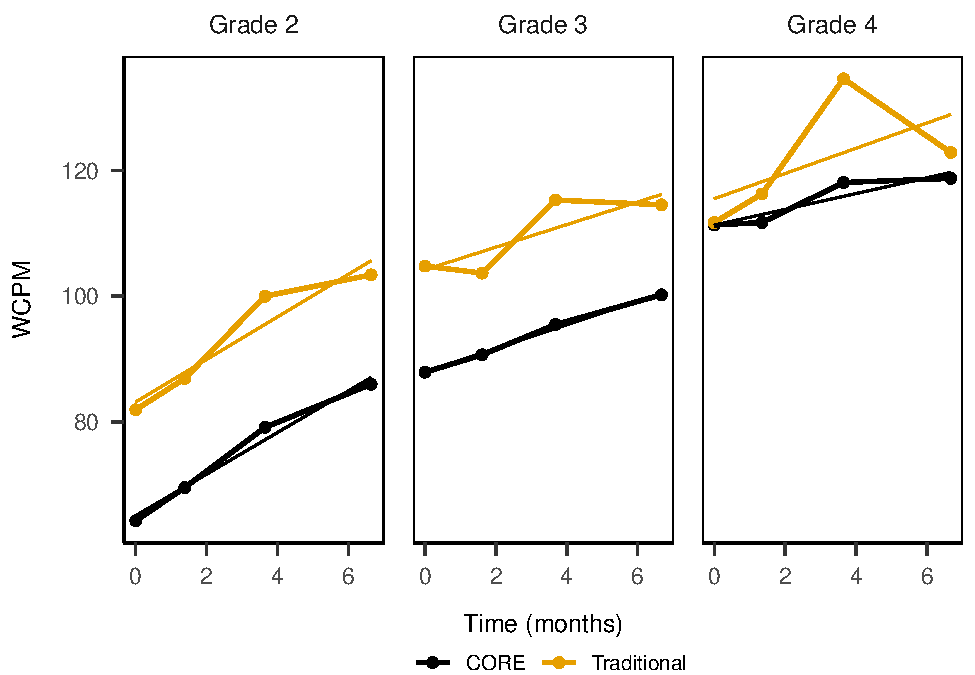
\includegraphics{conseq_validity_manusript_files/figure-latex/fig-means-1.pdf}
\caption{\label{fig:fig-means}Mean words correct per minute (WCPM) score across waves by grade and CBM-R measure.}
\end{figure}

\textbf{\emph{ASR Scoring.}} The ASR engine scored each audio recording file (both CORE and Traditional CBM-R), scoring each word as read correctly or incorrectly, and recording the time in centi-seconds to read each word and the time between words. Bavieca, an open-source speech recognition toolkit, was the ASR applied in this study (\url{http://www.bavieca.org/}). Bavieca uses continuous density hidden Markov models and supports maximum likelihood linear regression, vocal tract length normalization, and discriminative training (maximum mutual information). It uses the general approach of many state-of-the art speech recognition systems: a Viterbi Beam Search used to find the optimal mapping of the speech input onto a sequence of words. The score for a word sequence was calculated by interpolating language model scores and acoustic model scores. The language model assigned probabilities to sequences of words using trigrams (where the probability of the next word is conditioned on the two previous words) and was trained using the CMU-Cambridge LM Toolkit (Clarkson \& Rosenfeld, 1997). Acoustic models were clustered triphones based on Hidden Markov Models using Gaussian Mixtures to estimate the probabilities of the acoustic observation vectors. The system used filler models to match the types of disfluencies found in applications.

\hypertarget{reading-comprehension}{%
\subsubsection{Reading Comprehension}\label{reading-comprehension}}

The easyCBM reading comprehension measure assesses students comprehension of a 1,500 word fictional narrative. The comprehension items are designed to target students' literal, inferential, and evaluative comprehension. Split-half reliability ranged from .38 to .87, item reliability from Rasch analyses ranged from .39 to .94, and Cronbach's alpha ranged from .69 to .78 (Saez et al., 2010). Predictive (fall) and concurrent (spring) correlations between Grade 2 comprehension and spring SAT-10 reading scale scores were .62 and .66 respectively (Jamgochian et al., 2010). Predictive (fall) and concurrent (spring) correlations between Grade 3 and 4 comprehension and spring state reading test scores (Oregon Assessment of Knowledge and Skills {[}OAKS{]} and Washington Measures of Student Progress {[}MSP{]}) were .52 to .70, and .37 to .68 respectively (Anderson et al., 2014). Predictive diagnostic statistics for fall comprehension and spring state reading test scores included sensitivity from .68 to .86, specificity from .57 to .92, and AUC from .74 to .86. Concurrent diagnostic statistics for spring comprehension and spring state reading test scores included sensitivity from .69 to .89, specificity from .63 to .80, and AUC ranged from .76 to .87 (Anderson et al., 2014).

The Grade 2 comprehension measure contained 12 multiple-choice items (\emph{M} = 10.40, \emph{SD} = 1.70), whereas the Grade 3 (\emph{M} = 14.10, \emph{SD} = 4.10) and Grade 4 (\emph{M} = 13.50, \emph{SD} = 3.80) measures contained 20 multiple-choice items. Figure~\ref{fig:fig-comp-scatter} shows scatter plots of the CBM-R WCPM and comprehension scores by grade and season (distal and proximal).



\begin{figure}
\centering
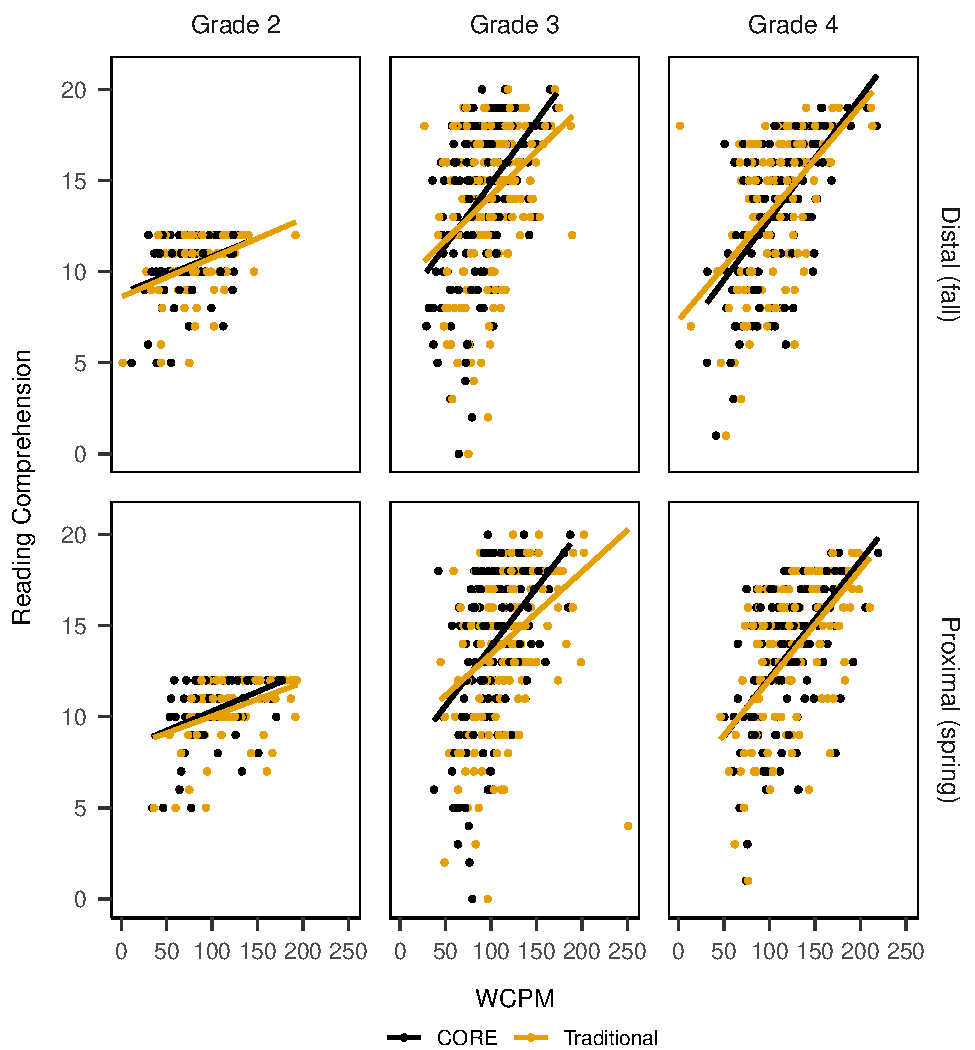
\includegraphics{conseq_validity_manusript_files/figure-latex/fig-comp-scatter-1.pdf}
\caption{\label{fig:fig-comp-scatter}Words correct per minute (WCPM) and comprehension scores by grade and season, distal (fall) and proximal (spring).}
\end{figure}

\hypertarget{sbac-reading-test}{%
\subsubsection{SBAC Reading Test}\label{sbac-reading-test}}

The Smarter Balanced Assessment Consortium (SBAC) English language arts/literacy (ELA/L) summative assessment is administered to students in Grades 3 through 8 and 11 and consists of two parts: a computerized adaptive test (CAT), and a performance task (PT) component. The SBAC ELA/L was developed to align to the Common Core State Standards (CCSS) and measures four broad claims: reading, writing, listening, and research (Consortium, 2020). Within each claim there are a number of assessment targets, and each test item is aligned to a specific claim and target and to a CCSS. The CAT consisted of selected response items that assess all four claims. The PT consisted of a set of related stimuli presented with two or three research items requiring both short-text responses and a full written response that assess the writing and research claims. The overall SBAC ELA/L performance scaled score is divided into four proficiency categories (\emph{Well Below}, \emph{Below}, \emph{Proficient}, and \emph{Advanced}), where the first two categories represent students who do not meet state grade-level reading achievement standards, and the last two categories represent students who do meet those standards.

The mean SBAC ELA/L score for Grade 3 was 2447 (\emph{SD} = 74.8) with 61\% meeting proficiency. The mean SBAC ELA/L score for Grade 4 was 2480 (\emph{SD} = 79.7) with 57\% meeting proficiency. Figure~\ref{fig:fig-sbac-scatter} shows scatter and density plots of the CBM-R WCPM and SBAC ELA/L score and proficiency, respectively, by grade and season (distal and proximal).



\begin{figure}
\centering
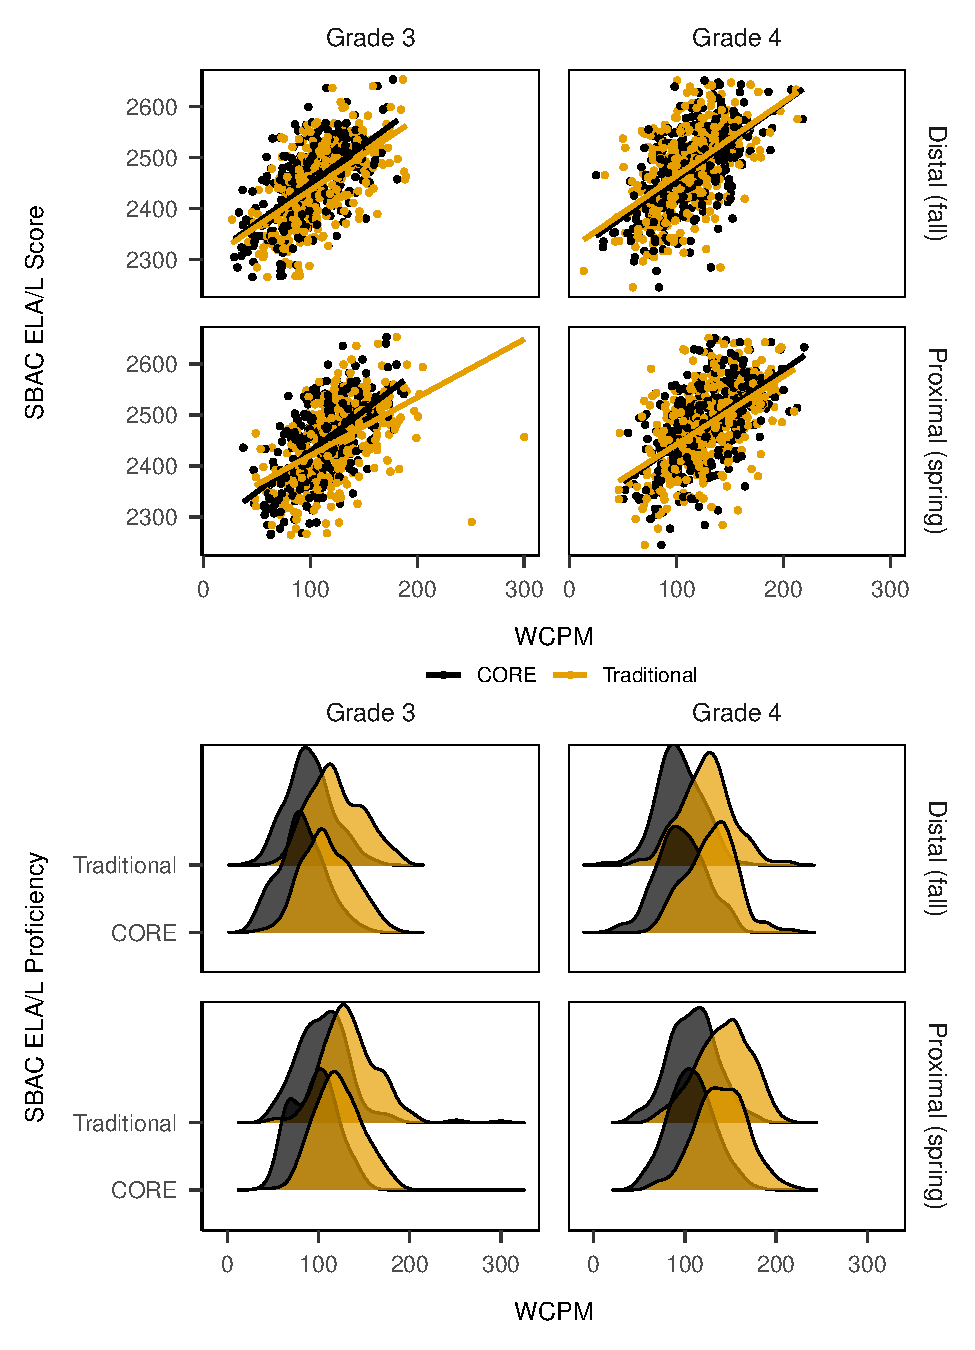
\includegraphics{conseq_validity_manusript_files/figure-latex/fig-sbac-scatter-1.pdf}
\caption{\label{fig:fig-sbac-scatter}Words correct per minute (WCPM) and SBAC ELA/L Score \& Proficiency classification by grade and season, distal (fall) and proximal (spring).}
\end{figure}

\hypertarget{procedure}{%
\subsection{Procedure}\label{procedure}}

Students were assessed online, using classroom or school devices, and wore headphones with an attached noise-canceling microphone provided by the research team. Students were introduced to the task by their teacher, and then directed to the study website where the first page asked for student assent (if a student declined, their participation ended). The standardized instructions were presented via audio as well as print. \emph{Get ready! You are about to do some reading! After pressing start, read the story on the screen. When you are finished click done. Do your best reading, and have fun!}

For each of the four measurement occasions (Oct-Nov 2017, 2018; Nov-Feb 2017-18, 2018-19; Feb-Mar 2018, 2019; May-Jun, 2018, 2019), students read aloud online a randomly assigned, fixed set of 10 to 12 CORE passages (3-5 long and 5-7 medium), and one Traditional CBM-R passage from the easyCBM progress monitoring system. The automatic speech recognition engine scored each reading, scoring each word as read correctly or incorrectly (accuracy), and recording the time duration to read each word and the silence between which was aggregated to calculate the time to read the passage (speed).

All WCPM scores were based on these readings and data. The model-based WCPM CORE scores (Kara, Kamata, Potgieter, \& Nese, 2020) were estimated for each measurement occasion based on the CORE passages. Traditional CBM-R WCPM scores were calculated by dividing the number of words read correctly (wrc) by the quotient of the total seconds read (s) and 60; that is, \(wrc/(s/60)\).

\hypertarget{analyses}{%
\subsection{Analyses}\label{analyses}}

All analyses and figures were conducted and created in the R programming environment (R Core Team, 2020) with the following R packages: effectsize (Ben-Shachar, Lüdecke, \& Makowski, 2020), doParallel (Corporation \& Weston, 2020), ggridges (Wilke, 2021), ggthemes (Arnold, 2021), janitor (Firke, 2021), lavaan (Rosseel, 2012), papaja (Aust \& Barth, 2020), patchwork (Pedersen, 2020), tidymodels (Kuhn \& Wickham, 2020); tidyverse (Wickham et al., 2019).

\textbf{\emph{Growth}}

To address RQ 1, we applied a latent growth model {[}LGM; Meredith and Tisak (1990){]} separately for each grade to represent students' within-year oral reading fluency growth. The slope factor loadings were specified as the elapsed number of months between the median month of wave 1 (\(t_1\)) and the median month at each wave \(t\) (see Table~\ref{tab:tbl-desc}). Two results are extracted from the LGMs to compare the growth properties of the traditional CBM-R and model-based CORE scores.

One, the standard error (\emph{SE}) of individual slope estimates, based on the latent intercept and slope factor scores as estimated by the LGM. The \emph{SE} of the slope estimate quantifies the variability, or precision, of the slope estimate that has been often used in CBM-R research (e.g., Ardoin \& Christ, 2009) to evaluate the accuracy of growth estimates. The \emph{SE} of slope for each student (\(SEb_i\)) is:
\[
SEb_i = \frac{\sqrt\frac{\Sigma(Y_i - \bar{Y})^2}{n - 2}}{\sqrt{\Sigma(t_i - \bar{t})^2}}
\]
where the numerator is the residual variance and the denominator is the square root of the sum, over the \(t\) waves, of the squared deviations of \(t_i\) about their mean (where \(t_i\) are the slope factor loadings).

Two, the reliability of the CBM-R scores at each wave, as estimated by the proportion of true score variance to observed score variance (Rogosa \& Willett, 1983; Singer, Willett, Willett, \& others, 2003; Willett, 1988):
\[
\rho_t = \frac{\psi_{00} + \lambda^2_t \psi_{11} + 2\lambda_t \psi_{01}}{\psi_{00} + \lambda^2_t \psi_{11} + 2\lambda_t \psi_{01} + \theta_t} = \frac{var(y_t) - \theta_t}{var(y_t)}
\]
where \(\rho_t\) represent the reliability at wave \(t\), \(\psi\) represents the covariance structure of the intercept and slope factors, \(\lambda_t\) represents the linear time covariate, and \(\theta_t\) represents the residual variance at a wave, which is equivalent to the ratio of the true score variance (\(var(y_t) - \theta_t\)) to the observed score variance (\(var(y_t)\)), and can be calculated for each wave by subtracting the residual variance (measurement error) from the observed score variance. This estimate of reliability provides both the true score variance explained by the longitudinal model and the unique measurement error variance of observed scores at each wave, and has been applied for estimating reliability of CBM data (Yeo, Kim, Branum-Martin, Wayman, \& Espin, 2012).

The LGM analyses were conducted using the lavaan package with maximum likelihood estimation with robust Huber-White standard errors and a scaled test statistic that is asymptotically equal to the Yuan-Bentler test statistic (Rosseel, 2012). This estimator is robust to non-normality and clustering (McNeish, Stapleton, \& Silverman, 2017).

\textbf{\emph{Predictive Performance}}

To address RQs 2 and 3, we apply a predictive approach to determine which CBM-R predictor most accurately estimates the outcomes, rather than an inferential approach that pursues unbiased estimates of \(\beta\) coefficients. Our predictive model is a linear model, separate for each grade and CBM-R predictor, regressing the spring outcome (comprehension, SBAC ELA/L scores, or SBAC ELA/L proficiency) on the CBM-R predictor (Traditional CBM-R scores or CORE model-based scores, fall or spring).

For RQ 2, we fit 12 linear models: two CBM-R predictors each at two seasons (fall and spring) for each of three grades: \(Comprehension_i = \beta_0 + \beta_1CBM\mbox{-}R_{season} + \epsilon_i\).

For RQ 3, we model Grades 3 and 4 together and thus included grade level as a categorical covariate, as well as the state (OR or WA) to account for differences in state standards. We fit eight linear models, applying a logistic regression for the categorical SBAC ELA/L proficiency outcome: \(SBAC_i = \beta_0 + \beta_1CBM\mbox{-}R_{season} + Grade + State + \epsilon_i\).

To measure the predictive performance of the models, \emph{RMSEA} and \(R^2\) were used for the continuous outcomes (spring comprehension and SBAC ELA/L scores), and the sensitivity, specificity, and Receiver Operating Characteristic (ROC) area under the curve (AUC) for the categorical outcome (SBAC ELA/L proficiency).

To understand the predictive performance of the CBM-R measures, and how that might generalize to new data, the data for each RQ were split into two sets: a training set, a random sample of 75\% of the data; and a testing set, the remaining 25\% of the data.

To get a measure of variance for the performance measures, 10-fold cross-validation was applied to the training set (Kuhn, Johnson, \& others, 2013). For each fold, 10\% of the training set is sampled and serves as an assessment sample, so that each observation serves in one and only one assessment sample. The remaining 90\% of the training set serve as the analysis sample for a fold. The predictive model is fit on the 90\% analysis sample of each fold, and the resulting model parameters are used to predict the assessment sample within each fold. The mean and \emph{SD} of the performance measures (\emph{RMSEA}, \(R^2\), sensitivity, specificity, and AUC) across the 10 folds are reported.

Research has shown that 10 folds is a sensible value for \emph{k}-fold cross-validation, and repeating \emph{k}-fold cross-validation can improve the performance of the estimates while maintaining small bias, particularly for smaller sample sizes (Kim, 2009; Molinaro, Simon, \& Pfeiffer, 2005). Thus, 10-fold cross-validation repeated five times was applied for each RQ training set so that 50 models were fit and 50 values of each performance measure were recorded (10 folds \(\times\) 5 repeats = 50 models).

Finally, the predictive models were fit to the entire training set, and then the resulting model parameters were used to predict the test set. The test set here can be can be conceptualized as ``new'' (or unseen) data, as it has not been used in the model parameter estimation. The resulting final performance measures serve as estimates of how the two comparison CBM-R measures might generalize in their predictive performance. The predictive modeling process was conducted using the tidymodels package (Kuhn \& Wickham, 2020).

\hypertarget{results}{%
\section{Results}\label{results}}

Figure~\ref{fig:fig-means} shows the difference between CORE and Traditional CBM-R in mean WCPM scores across grades and waves. The CORE trajectories were smoother than Traditional CBM-R, visually demonstrating more reliability in scores. In addition, the mean CORE scores were consistently and meaningfully lower than the mean Traditional CBM-R scores.

\hypertarget{rq1}{%
\subsection{RQ1}\label{rq1}}

To address RQ 1, we fit LGMs separately for each CBM-R measure and grade. The fit measures for the Grade 2 CORE LGM were \(\chi^2\) = 13.70 with \emph{df} = 5 (\emph{p} = .018), Tucker Lewis Index (TLI) = 1, Comparative Fit Index (CFI) = 1, \emph{RMSEA} = 0.04, and BIC = 17,986.3. The fit measures for the Grade 2 Traditional CBM-R LGM were \(\chi^2\) = 56.40 with \emph{df} = 5 (\emph{p} \textless{} .001), TLI = 0.93, CFI = 0.94, \emph{RMSEA} = 0.13, and BIC = 13,647.1. The fit measures for the Grade 3 CORE LGM were \(\chi^2\) = 9.20 with \emph{df} = 5 (\emph{p} = .100), TLI = 1, CFI = 1, \emph{RMSEA} = 0.03, and BIC = 23,365.1. The fit measures for the Grade 3 Traditional CBM-R LGM were \(\chi^2\) = 65.10 with \emph{df} = 5 (\emph{p} \textless{} .001), TLI = 0.96, CFI = 0.96, \emph{RMSEA} = 0.11, and BIC = 19,956.8. The fit measures for the Grade 4 CORE LGM were \(\chi^2\) = 28.50 with \emph{df} = 5 (\emph{p} \textless{} .001), TLI = 0.99, CFI = 0.99, \emph{RMSEA} = 0.08, and BIC = 21,461.1)`.

The Grade 4 LGM for Traditional CBM-R was not successfully estimated without a negative variance for the slope factor. We tried alternate modeling solutions, including homogeneous residual variances (and zero error covariances), heterogeneous Toeplitz residual structure, first-order autocorrelated residuals (McNeish \& Harring, 2019), and transformed slope factor loadings, but all models were unsuccessful due to a negative variance or variance-covariance matrix. Thus, we do not report the results from this model. All of the parameter estimates from the LGMs can be found in the Appendix (Table~\ref{tab:tbl-lgms-results}).

Table~\ref{tab:tbl-seb-results} shows the mean (\emph{SD}) of the standard error of the individual slope estimates (\(SEb\)) by measure and grade. Across grades, the mean \(SEb\) for the model-based CORE models (range = 2.82 to 3.16) were smaller than the Traditional CBM-R models (3.93 and 4.32). To give context to these mean differences, Cohen's \emph{d} (1988) was calculated as a standardized mean difference effect sizes statistic, and \emph{d} = 0.41 and 0.55 for Grades 2 and 3 respectively, both of which can be classified as large in magnitude (Kraft, 2020; Lipsey et al., 2012). In addition, the \emph{SD}s of the CORE \(SEb\)s were smaller by 22\% and 30\%, indicating more precision spread in these estimated for CORE compared to Traditional CBM-R.

Table~\ref{tab:tbl-lgms-reliab} shows the observed variances of the CBM-R measures at each wave, the estimated residual variances from the LGMs, and reliability estimates by grade and wave. Across grades and waves, the reliability estimates were higher for the model-based CORE scores except for Grade 2, wave 4 (.85 vs.~.86). The reliability estimates for the model-based CORE scores ranged from .82 to .93, and for the Traditional CBM-R ranged from .62 to .86. Using Cohen's \emph{h} (1988) as a measure of distance between two proportions (i.e., true score variance explained), the differences in the reliability estimates can be interpreted similarly to effect sizes, where the Grade 2 wave 4 difference favoring Traditional CBM-R is near zero, and the remaining differences favoring CORE range from \emph{h} = .11 to .52, which can be classified as small to medium in magnitude (Cohen, 1988).



\begin{table}[tbp]

\begin{center}
\begin{threeparttable}

\caption{\label{tab:tbl-seb-results}Mean (SD) of the Standard Error of the Slope (SEb) Estimate by Measure and Grade.}

\begin{tabular}{lrrrrrr}
\toprule
 & \multicolumn{2}{c}{CORE} & \multicolumn{2}{c}{Traditional}  &  &\\
\cmidrule(r){2-3} \cmidrule(r){4-5}
Grade & \multicolumn{1}{c}{Mean \emph{SEb}} & \multicolumn{1}{c}{\emph{SD}} & \multicolumn{1}{c}{Mean \emph{SEb}} & \multicolumn{1}{c}{\emph{SD}} & \multicolumn{1}{c}{\emph{d}} & \multicolumn{1}{c}{CI}\\
\midrule
2 & 2.82 & (2.36) & 3.93 & (3.04) & 0.41 & {}[0.29 - 0.53]\\
3 & 2.88 & (2.36) & 4.32 & (3.38) & 0.55 & {}[0.45 - 0.65]\\
4 & 3.16 & (2.46) & -- & -- & -- & --\\
\bottomrule
\addlinespace
\end{tabular}

\begin{tablenotes}[para]
\normalsize{\textit{Note.} d = Cohen's d (1988). CI = 95\% confidence interval.}
\end{tablenotes}

\end{threeparttable}
\end{center}

\end{table}



\begin{center}
\begin{ThreePartTable}

\begin{longtable}{lrrrrrrl}\noalign{\getlongtablewidth\global\LTcapwidth=\longtablewidth}
\caption{\label{tab:tbl-lgms-reliab}Observed Variances, Estimated Residual Variances, and Reliability Estimates by Grade and Wave.}\\
\toprule
 & \multicolumn{3}{c}{CORE} & \multicolumn{3}{c}{Traditional}  &\\
\cmidrule(r){2-4} \cmidrule(r){5-7}
Wave & \multicolumn{1}{c}{Observed} & \multicolumn{1}{c}{Residual} & \multicolumn{1}{c}{Reliability} & \multicolumn{1}{c}{Observed} & \multicolumn{1}{c}{Residual} & \multicolumn{1}{c}{Reliability} & \multicolumn{1}{c}{\emph{h}}\\
\midrule
\endfirsthead
\caption*{\normalfont{Table \ref{tab:tbl-lgms-reliab} continued}}\\
\toprule
 & \multicolumn{3}{c}{CORE} & \multicolumn{3}{c}{Traditional}  &\\
\cmidrule(r){2-4} \cmidrule(r){5-7}
Wave & \multicolumn{1}{c}{Observed} & \multicolumn{1}{c}{Residual} & \multicolumn{1}{c}{Reliability} & \multicolumn{1}{c}{Observed} & \multicolumn{1}{c}{Residual} & \multicolumn{1}{c}{Reliability} & \multicolumn{1}{c}{\emph{h}}\\
\midrule
\endhead
Grade 2 &  &  &  &  &  &  & \\
\ \ \ Wave 1 & 1185.0 & 108.2 & .91 & 802.2 & 174.9 & .78 & .36\\
\ \ \ Wave 2 & 1176.9 & 123.3 & .90 & 973.5 & 170.1 & .83 & .20\\
\ \ \ Wave 3 & 1211.5 & 188.1 & .84 & 1010.1 & 383.2 & .62 & .52\\
\ \ \ Wave 4 & 1100.1 & 166.3 & .85 & 1167.2 & 164.7 & .86 & -.03\\
Grade 3 &  &  &  &  &  &  & \\
\ \ \ Wave 1 & 1239.5 & 86.3 & .93 & 1010.9 & 211.1 & .79 & .42\\
\ \ \ Wave 2 & 1226.5 & 171.0 & .86 & 1164.1 & 345.3 & .70 & .39\\
\ \ \ Wave 3 & 1221.7 & 175.8 & .86 & 1242.2 & 325.1 & .74 & .30\\
\ \ \ Wave 4 & 1052.1 & 173.1 & .84 & 1190.4 & 245.0 & .79 & .11\\
Grade 4 &  &  &  &  &  &  & \\
\ \ \ Wave 1 & 1197.9 & 103.9 & .91 & -- & -- & -- & --\\
\ \ \ Wave 2 & 1280.1 & 167.6 & .87 & -- & -- & -- & --\\
\ \ \ Wave 3 & 1173.7 & 149.5 & .87 & -- & -- & -- & --\\
\ \ \ Wave 4 & 1147.9 & 207.4 & .82 & -- & -- & -- & --\\
\bottomrule
\end{longtable}

\end{ThreePartTable}
\end{center}

\hypertarget{rq2}{%
\subsection{RQ2}\label{rq2}}

For RQ 2 we compared the predictive performance of CORE and Traditional CBM-R for distal (fall) and proximal (spring) assessments predicting spring comprehension scores for students in Grades 2 through 4. Table~\ref{tab:tbl-pred-comp} shows the mean \emph{RMSE} and \(R^2\) values across the 50 models fit to the 10-fold cross-validation samples, as well as the final \emph{RMSE} and \(R^2\) values for the full training/testing samples. To give context to the \emph{RMSE} values, the comprehension assessment had 12 items for Grade 2 and 20 items for Grades 3 and 4, with \emph{SD}s of 1.69, 4.06, and 3.80, respectively, so the \emph{RMSE} values were generally smaller than the sample \emph{SD}s.

For the cross-validation, the distal (fall) and proximal (spring) CBM-R predictor results generally favored CORE which had better (lower) mean \emph{RMSE} values compared to Traditional CBM-R, and better (higher) mean \(R^2\) values, except Grade 2 and Grade 4 proximal. The standardized mean differences in \emph{RMSE} for distal results across grades were \(d\) = -0.08, 0.25, and 0.45, and for proximal were 0.00, 0.29, and -0.08. The standardized mean differences in \(R^2\) for distal were \(h\) = 0.00, 0.12, and 0.19, and for proximal were 0.00, 0.09, and -0.02 (Cohen, 1988). In addition, the \emph{SD}s of the \emph{RMSE} estimates favored CORE by 2\% to 75\%, except Grade 2 distal (-8\%) and Grade 4 proximal (-9\%), and the \emph{SD}s of the \(R^2\) estimates favored CORE by 5\% to 17\%, except Grade 2 proximal (-4\%) and Grades 2 and 3 distal which were the same across measures. These results suggest somewhat less spread in the performance measure estimates for CORE compared to Traditional CBM-R.

The final \emph{RMSE} and \(R^2\) values in Table~\ref{tab:tbl-pred-comp} represent the parameters of the predictive models fit to the training set (75\% of sample) and then used to predict the testing set (25\% of sample). The results generally favored CORE, which had lower \emph{RMSE} and higher \(R^2\) values except Grade 3 proximal \emph{RMSE}. The \emph{RMSE} values represent differences of 1\% to 11\% of a \emph{SD} favoring CORE, and -2\% of a \emph{SD} favoring Traditional CBM-R for the Grade 3 proximal model. The \(R^2\) values represent increases in explained variance for CORE above Traditional CBM-R of 1\% to 13\%. The standardized mean differences in \(R^2\) all favored CORE, with \(h\) = 0.08 , 0.46, and 0.03 across grades for the distal models, and 0.12, 0.01, and 0.11 for the proximal models (Cohen, 1988).



\begin{lltable}

\small{

\begin{longtable}{lrrrrrrrrrrrr}\noalign{\getlongtablewidth\global\LTcapwidth=\longtablewidth}
\caption{\label{tab:tbl-pred-comp}Spring Comprehension Predictive Measures (RMSE and R2) For Distal and Proximal CBM-R Predictors by Grade.}\\
\toprule
 & \multicolumn{6}{c}{CORE} & \multicolumn{6}{c}{Traditional} \\
\cmidrule(r){2-7} \cmidrule(r){8-13}
Grade & \multicolumn{1}{c}{Mean \emph{RMSE}} & \multicolumn{1}{c}{(\emph{SD})} & \multicolumn{1}{c}{Mean $R^2$} & \multicolumn{1}{c}{(\emph{SD})} & \multicolumn{1}{c}{Final \emph{RMSE}} & \multicolumn{1}{c}{Final $R^2$} & \multicolumn{1}{c}{Mean \emph{RMSE}} & \multicolumn{1}{c}{(\emph{SD})} & \multicolumn{1}{c}{Mean $R^2$} & \multicolumn{1}{c}{(\emph{SD})} & \multicolumn{1}{c}{Final \emph{RMSE}} & \multicolumn{1}{c}{Final $R^2$}\\
\midrule
\endfirsthead
\caption*{\normalfont{Table \ref{tab:tbl-pred-comp} continued}}\\
\toprule
 & \multicolumn{6}{c}{CORE} & \multicolumn{6}{c}{Traditional} \\
\cmidrule(r){2-7} \cmidrule(r){8-13}
Grade & \multicolumn{1}{c}{Mean \emph{RMSE}} & \multicolumn{1}{c}{(\emph{SD})} & \multicolumn{1}{c}{Mean $R^2$} & \multicolumn{1}{c}{(\emph{SD})} & \multicolumn{1}{c}{Final \emph{RMSE}} & \multicolumn{1}{c}{Final $R^2$} & \multicolumn{1}{c}{Mean \emph{RMSE}} & \multicolumn{1}{c}{(\emph{SD})} & \multicolumn{1}{c}{Mean $R^2$} & \multicolumn{1}{c}{(\emph{SD})} & \multicolumn{1}{c}{Final \emph{RMSE}} & \multicolumn{1}{c}{Final $R^2$}\\
\midrule
\endhead
Distal &  &  &  &  &  &  &  &  &  &  &  & \\
\ \ \ Grade 2 & 1.30 & 0.50 & 0.27 & 0.25 & 2.14 & 0.07 & 1.26 & 0.46 & 0.27 & 0.25 & 2.15 & 0.05\\
\ \ \ Grade 3 & 3.48 & 0.55 & 0.26 & 0.17 & 3.90 & 0.17 & 3.62 & 0.57 & 0.21 & 0.17 & 4.36 & 0.04\\
\ \ \ Grade 4 & 2.92 & 0.67 & 0.36 & 0.23 & 3.05 & 0.48 & 3.25 & 0.78 & 0.27 & 0.19 & 3.16 & 0.46\\
Proximal &  &  &  &  &  &  &  &  &  &  &  & \\
\ \ \ Grade 2 & 1.27 & 0.52 & 0.32 & 0.27 & 2.07 & 0.17 & 1.27 & 0.53 & 0.32 & 0.28 & 2.10 & 0.12\\
\ \ \ Grade 3 & 3.43 & 0.53 & 0.28 & 0.16 & 4.21 & 0.08 & 3.65 & 0.93 & 0.24 & 0.15 & 4.12 & 0.08\\
\ \ \ Grade 4 & 3.08 & 0.65 & 0.31 & 0.20 & 3.10 & 0.46 & 3.03 & 0.59 & 0.32 & 0.19 & 3.25 & 0.41\\
\bottomrule
\end{longtable}

}

\end{lltable}

\hypertarget{rq3}{%
\subsection{RQ3}\label{rq3}}

For RQ 3 we compared the predictive performance of CORE and Traditional CBM-R for distal (fall) and proximal (spring) assessments predicting spring SBAC ELA/L (scores and proficiency classification) for students in Grades 3 and 4. Table~\ref{tab:tbl-pred-sbac} shows the mean \emph{RMSE}, \(R^2\), sensitivity, specificity, and AUC values across the 50 models fit to the 10-fold cross-validation samples, as well as the final \emph{RMSE}, \(R^2\), sensitivity, specificity, and AUC values for the training/testing samples. To give context to the \emph{RMSE} values, the \emph{SD} of SBAC ELA/L was 79.03 for Grades 3 and 4 combined.

For the SBAC ELA/L score (continuous) outcome, both the distal and proximal results favored CORE which had lower mean and final \emph{RMSE} and higher mean and final \(R^2\) values across grades compared to Traditional CBM-R. The standardized mean differences in \emph{RMSE} were \(d\) = 0.27 (distal) and 0.59 (proximal), and in \(R^2\) were \(h\) = 0.06 (distal) and 0.14 (proximal), showing larger effects for proximal models. In addition, the \emph{SD}s of the performance measures were smaller for CORE by 9\% to 31\% (except for distal \(R^2\)), indicating less spread in these measures compared to Traditional CBM-R. The final \emph{RMSE} and \(R^2\) values in Table~\ref{tab:tbl-pred-sbac} (representing the training/testing sets) favored CORE for both distal and proximal models, with reductions in \emph{RMSE} of 2\% and 3\%, and reductions in \(R^2\) of 9\% and 16\%, which correspond to standardized differences of \(h\) = 0.07 and 0.13 (Cohen, 1988).

The results of SBAC ELA/L proficiency (classification) outcome also favored CORE. For the cross-validation, the distal predictors, CORE had lower mean sensitivity (\(d\) = 0.06), mean specificity (\(d\) = 0.08), and mean AUC (\(d\) = 0.05), and for the proximal predictors, CORE had lower mean sensitivity (\(d\) = 0.04), higher mean specificity (\(d\) = -0.05), and mean AUC (0.81) was the same across measures. In addition, the \emph{SD}s of the performance measures estimates favored CORE by 9\% to 75\%, indicating less spread in the performance measure estimates for CORE compared to Traditional CBM-R (the \emph{SD} of specificity for the proximal models were the same across measures). The final results of the training/testing sets favored CORE for both distal and proximal models, with final distal sensitivity the same across measures (0.51), but lower final proximal sensitivity by 4\%, lower final specificity (8\% distal, 3\% proximal), and lower final AUC (3\% distal, 4\% proximal).



\begin{center}
\begin{ThreePartTable}

\begin{longtable}{lll}\noalign{\getlongtablewidth\global\LTcapwidth=\longtablewidth}
\caption{\label{tab:tbl-pred-sbac}Predictive Performance Measures by Distal and Proximal CBM-R Predictors and Outcome (SBAC ELA/L Score and Proficiency).}\\
\toprule
Performance Measure & \multicolumn{1}{c}{CORE} & \multicolumn{1}{c}{Traditional}\\
\midrule
\endfirsthead
\caption*{\normalfont{Table \ref{tab:tbl-pred-sbac} continued}}\\
\toprule
Performance Measure & \multicolumn{1}{c}{CORE} & \multicolumn{1}{c}{Traditional}\\
\midrule
\endhead
Distal - SBAC Score &  & \\
\ \ \ Mean \emph{RMSE} (\emph{SD}) & 61.62 (5.80) & 63.26 (6.35)\\
\ \ \ Mean $R^2$ (\emph{SD}) & 0.41 (0.08) & 0.38 (0.08)\\
\ \ \ Final \emph{RMSE} & 58.53 & 60.03\\
\ \ \ Final $R^2$ & 0.40 & 0.37\\
Proximal - SBAC Score &  & \\
\ \ \ Mean \emph{RMSE} (\emph{SD}) & 61.57 (5.94) & 65.63 (7.80)\\
\ \ \ Mean $R^2$ (\emph{SD}) & 0.41 (0.09) & 0.34 (0.10)\\
\ \ \ Final \emph{RMSE} & 59.35 & 61.90\\
\ \ \ Final $R^2$ & 0.39 & 0.33\\
Distal - SBAC Proficiency &  & \\
\ \ \ Mean Sensitivity (\emph{SD}) & 0.62 (0.10) & 0.59 (0.11)\\
\ \ \ Mean Specificity (\emph{SD}) & 0.83 (0.07) & 0.80 (0.08)\\
\ \ \ Mean AUC (\emph{SD}) & 0.81 (0.05) & 0.79 (0.06)\\
\ \ \ Final Sensitivity & 0.51 & 0.51\\
\ \ \ Final Specificity & 0.86 & 0.79\\
\ \ \ Final AUC & 0.79 & 0.76\\
Proximal - SBAC Proficiency &  & \\
\ \ \ Mean Sensitivity (\emph{SD}) & 0.63 (0.10) & 0.61 (0.11)\\
\ \ \ Mean Specificity (\emph{SD}) & 0.80 (0.07) & 0.82 (0.07)\\
\ \ \ Mean AUC (\emph{SD}) & 0.81 (0.05) & 0.81 (0.06)\\
\ \ \ Final Sensitivity & 0.57 & 0.54\\
\ \ \ Final Specificity & 0.86 & 0.83\\
\ \ \ Final AUC & 0.79 & 0.76\\
\bottomrule
\end{longtable}

\end{ThreePartTable}
\end{center}

\hypertarget{discusion}{%
\section{Discusion}\label{discusion}}

CBM-R, administered in classrooms across the country, is used as an indicator of reading proficiency, and to measure at risk students' response to reading interventions to help ensure instruction is effective. As such, CBM-R scores need to be predictive of reading comprehension and year-end state test scores/proficiency, and sufficiently reliable so educators to make inferences about students' response to intervention. The present study compared traditional CBM-R WCPM scores with model-based WCPM scores to examine their consequential validity properties for students in Grades 2 through 4, including reliability and predictive performance, to evaluate CORE's utility as a CBM-R assessment for both progress monitoring and screening.

The CORE trajectories were not only less variant than those of the Traditional CBM-R, the mean CORE scores were consistently and meaningfully lower than the mean Traditional CBM-R scores (Figure~\ref{fig:fig-means}). Thus, if the model-based CORE scores are interpreted as more reliable and precise, as the results suggest, then Traditional CBM-R WCPM scores tend to overestimate (on average) student oral reading fluency.

\hypertarget{within-year-growth-properties}{%
\subsection{Within-year Growth Properties}\label{within-year-growth-properties}}

In response to the first research question, the results of the LGMs showed, in general, better within-growth properties for the model-based CORE scores. The \emph{SD}s of the \(SEb\) estimates for the Traditional CBM-R LGMs were about 29\% to 43\% larger than those of the CORE CBM-R models, and the effect sizes associated with these reductions (\emph{d} = 0.41 and 0.55) were of a magnitude that represent meaningful and promising significance (Table~\ref{tab:tbl-seb-results}). These results indicate that the individual slope parameter estimates for the CORE model-based scores were more precise than those of the traditional CBM-R scores. This precision is relevant for consequential validity and score-based educational decisions, as the model-based CBM-R scores should provide greater confidence in the progress monitoring decisions that are based on these scores than Traditional CBM-R.

The results of the LGMs also showed that the model-based CORE scores had higher reliability, as measured at each measurement occasion. The reliability estimates for the model-based CORE scores ranged from .82 to .93, and for the Traditional CBM-R ranged from .62 to .86. Excluding Grade 2 wave 4 where reliability favored Traditional CBM-R by .01 (\(h\) = -.03), the CORE reliability estimates were larger than the Traditional reliability estimates by .05 to .22, with medium to large associated standardized differences from \(h\) = .11 to .52. Thus, compared to Traditional CBM-R scores, a larger proportion of model-based CORE reliability is related to the estimate of true score variance and a smaller proportion is attributable to measurement error variance.

Based on the results of the LGMs (\(SEb\) \emph{SD} and reliability), and the model-based CORE scores demonstrated better measurement properties, or more precision, than Traditional CBM-R scores. Because reliability is inversely related with error variance, it can be inferred that CBM-R data with lower reliability exerts a negative influence over the estimated slope (Yeo, Kim, Branum-Martin, Wayman, \& Espin, 2012), which is an important part of identifying students at risk of poor reading outcomes, or those not adequately responding to reading instruction. For example, the correlation between the WCPM scores from wave 1 and wave 4 for Traditional CBM-R scores was \(r\) = 0.74, and for model-based CORE scores was \(r\) = 0.86, which helps demonstrate the increased precision of scores across time. Because the model-based CORE scores demonstrated higher reliability than Traditional CBM-R based on the LGMs, and the latent slope means were measured with less variance, it can be reasoned that the model-based CORE scores may yield growth estimates better suited to monitoring student oral reading fluency growth, and may provide better data with which to make instructional decisions, such as risk status or responsiveness to instruction.

In addition, the correlation between the latent intercept and slope factors for the CORE models were negative and moderate in magnitude, but were positive and small to moderate in magnitude for the traditional CBM-R models. These results may reflect of a ceiling effect, but that is not supported by the data; rather, these results suggest the model-based CORE scores are more sensitive to growth for students at risk of poor reading outcomes (i.e., lower fall WCPM scores), a finding that is supported by previous research that found increased precision (i.e., smaller conditional standard error of measurement) for CBM-R scores at/below the 25th percentile (Nese \& Kamata, 2020a). This finding should be further examined by future research.

Of critical importance to the inferences drawn from this study and for applied researchers, particularly those working for state or local education agencies and their data, is that we could not successfully estimate the Grade 4 Traditional CBM-R model, despite trying several different LGM specifications. The reason for this is unclear. It could be due to data missingness, but this is unlikely given that (a) the missingness was similar to those data of the other models, and (b) a model with no missing data was not estimated without negative variance. We speculate that the Grade 4 Traditional CBM-R model was not successfully estimated because of the large increase in scores at wave 3 (Figure~\ref{fig:fig-means}), which may be an artifact of large measurement error.

\hypertarget{predictive-performance}{%
\subsection{Predictive Performance}\label{predictive-performance}}

The results of the predictive modeling of the reading comprehension and SBAC ELA/L scores and proficiency showed that the model-based CORE scores had lower final \emph{RMSE} and higher final \(R^2\), sensitivity, specificity, and AUC values across all comparisons, grade and the distal (fall) and proximal (spring) CBM-R predictors (except comprehension Grade 3, proximal \emph{RMSE}; 4.12 vs.~4.21). The final performance measure values for these continuous outcomes in Table~\ref{tab:tbl-pred-comp} and Table~\ref{tab:tbl-pred-sbac} represent estimates of values that might be expected in new (or unseen) data, such as in future studies or in schools similar to those in this study. Thus, in general, model-based CORE scores showed better predictive performance in predicting year-end comprehension and state reading test scores than did Traditional CBM-R scores.

These comparative improvements in predictive performance ranged in magnitude. The final \emph{RMSE} values represented fairly modest gains of about 1\% to 11\% of a \emph{SD} for comprehension, and about 2\% of a \emph{SD} for SBAC scores. If these improvements were interpreted on a scale of effect sizes for education interventions, they would be considered small to medium in magnitude (Kraft, 2020). But in a predictive framework, any increase in predictive performance can be interpreted as a benefit, especially for the comprehension measures which had score ranges of 0 to 12 (Grade 2) or 0 to 20 (Grades 3 and 4). In addition, compared to Traditional CBM-R, the CORE final \(R^2\) values for comprehension represented an average gain of 4\%, and standardized differences of \(h\) = 0.01 to 0.46, and for SBAC scores \(h\) = 0.07 and 0.13, which could be considered meaningful benefits in explained variance for a single predictor.

Similarly for the SBAC ELA/L proficiency (classification) outcome, the results favored CORE with standardized differences of \(h\) = 0.00 and 0.05 for sensitivity, 0.18 and 0.08 for sensitivity, and 0.06 and 0.08 for AUC. Technical standards criterion for academic assessment screening measures indicate that the highest standard for AUC estimates are \(\geq\) .80, with specificity \(\geq\) .80 and sensitivity \(\geq\) .70 (\url{https://charts.intensiveintervention.org/ascreening}). The CORE distal (fall) and proximal (spring) measures nearly met the AUC standard with final values at .79, and both CORE predictors (.86) and one Traditional CBM-R predictor (.79 and .83) met the specificity standard. Neither CBM-R measure, however, meet the sensitivity standard.

It is desirable to have a test that has high sensitivity and specificity, but the two are generally inversely related such that as one increases, the other decreases. Both the CORE and Traditional CBM-R measures adequately predicted students that met year-end grade-level achievement standards (specificity), with low rates of false positives (i.e., incorrectly predicting students would not meet proficiency standards). This helps prevent over-identifying students at risk of poor reading outcomes, which helps school better allocate limited resources for reading intervention. But neither the CORE or the Traditional CBM-R measure adequately predicted students that did not meet year-end grade-level achievement standards (sensitivity), with higher than desirable rates of false negatives (i.e., correctly predicting students would not meet proficiency standards). The implications of lower sensitivity is that some students at risk of not meeting year-end proficiency standards are not identified, meaning that if the CBM-R measure was the only indicator of risk, these students would not receive the reading supports they need.

\hypertarget{limitations}{%
\subsection{Limitations}\label{limitations}}

There are several limitations in the present study that should be noted and considered when interpreting results. The consequential validity properties reported in response to the research questions generally reflect aspects of the samples and models applied, which may have implications for the interpretation and inferences of the results and the use of the CBM-R measures in specific contexts (Messick, 1995).

For the samples used here, the small sample sizes affect parameter estimation and potentially limit generalizations of the reported results. For example, the sample size used to answer RQ2 was small for each grade, but particularly for Grade 2 (Table~\ref{tab:tbl-demos}). Also, although the cross-validation models were repeated five times to to help improve performance for the smaller sample sizes (Kim, 2009; Molinaro, Simon, \& Pfeiffer, 2005), their results are likely to be susceptible to data-dependent variance. For the predictive models applied, the linear models are associated with high statistical bias (the difference between model predictions and the true values) and low variance (variability of a model prediction for a data point given new data); that is, linear regression is less prone to overfitting to the data, which may perhaps offer some protection against the small sample sizes. But future research needs to replicate this study with new data to explore reproducibility. Also, the reliability estimates of RQ1 are dependent on the specification of the LGM, and misspecification can affect estimates of parameters, but this would likely result in an underestimation of reliability and likely not affect the relative gains of CORE compared to the Traditional CBM-R measure (Yeo, Kim, Branum-Martin, Wayman, \& Espin, 2012).

The LGMs were fit to four waves of data that were intended to represent entire classrooms, making the measure more similar to (triannual) screening assessments, and less similar to progress monitoring data. Future research should extend this study and include a planned study with students receiving additional reading supports and their corresponding CBM-R progress monitoring data to examine the growth and reliability properties of model-based CORE scores. In addition, the CBM-R measures correlations with the continuous outcomes (Table~\ref{tab:tbl-cor}) were generally lower than reported average empirical correlations of CBM-R and reading comprehension on state achievement tests (\(r\) = .63; Shin and McMaster (2019)). As such, the analyses conducted in this study should be replicated with different samples, different traditional CBM-R measures, and different reading outcomes to explore the generalizability of results. Finally, the logistic regression classification threshold (.50) could be potentially be optimized to increase the accuracy of state-test proficiency predictions. While this may improve prediction performance, it would both CBM-R measures equally, and thus would not affect the results of the comparison between measures.

\hypertarget{conslusion}{%
\subsection{Conslusion}\label{conslusion}}

A simple interpretation of the results presented here is that the model-based CORE scores had a stronger relation with year-end reading comprehension and SBAC ELA/L scores, which has implications for educators using oral reading fluency measures for educational decisions. Good reading fluency has a theoretical and empirical relation with good reading comprehension, the latter of which is the ultimate goal of reading instruction. Descriptive analysis showed that the model-based CORE scores had higher correlations with both continuous outcomes across grades, except Grade 4, proximal (equal correlation) and Grade 2, distal (Table~\ref{tab:tbl-cor}). The model-based CORE scores, with a stronger relation with reading comprehension, can potentially better help with early identification of students at risk of poor reading outcomes and potentially better help monitor the reading fluency progress of those at-risk students because the scores provide a better estimate of students' current and prospective reading proficiency.

This study is an important part of a larger effort to improve traditional CBM-R assessment and the systems used by educators to make data-based decisions. CORE reshapes oral reading fluency and traditional CBM-R assessment by allowing group administration, more than one minute of reading, multiple passages, machine scoring, and WCPM scale scores. The benefits include reduced human administration cost and errors (Nese \& Kamata, 2020b), and reduced standard error of measurement (Nese \& Kamata, 2020a). The results of this study suggest increased measurement precision for the model-based CORE scores compared to traditional CBM-R, providing preliminary evidence that CORE can be used for consequential assessment. This is important for practitioners, as these measures are used to screen for students at risk of poor reading outcomes, and to monitor the progress of those students receiving reading intervention. CORE could provide more accurate data to predict which students may not meet state reading standards so that intervention could be delivered, and more precise data to evaluate the effectiveness of intervention and base educational decisions, such as determining whether the intervention is effective or needs to be modified to better meet the student's needs.

\newpage

\hypertarget{references}{%
\section{References}\label{references}}

\begingroup
\setlength{\parindent}{-0.5in}
\setlength{\leftskip}{0.5in}

\hypertarget{refs}{}
\begin{CSLReferences}{1}{0}
\leavevmode\hypertarget{ref-alonzotindal2007}{}%
Alonzo, J., \& Tindal, G. (2007). The development of word and passage reading fluency measures for use in a progress monitoring assessment system. Technical report\# 40. \emph{Behavioral Research and Teaching}.

\leavevmode\hypertarget{ref-anderson2014tech}{}%
Anderson, D., Alonzo, J., Tindal, G., Farley, D., Irvin, P. S., Lai, C.-F., \ldots{} Wray, K. A. (2014). Technical manual: easyCBM. Technical report\# 1408. \emph{Behavioral Research and Teaching}.

\leavevmode\hypertarget{ref-ardoin2009}{}%
Ardoin, S. P., \& Christ, T. J. (2009). Curriculum-based measurement of oral reading: Standard errors associated with progress monitoring outcomes from DIBELS, AIMSweb, and an experimental passage set. \emph{School Psychology Review}, \emph{38}(2), 266--283.

\leavevmode\hypertarget{ref-R-ggthemes}{}%
Arnold, J. B. (2021). \emph{Ggthemes: Extra themes, scales and geoms for 'ggplot2'}. Retrieved from \url{https://CRAN.R-project.org/package=ggthemes}

\leavevmode\hypertarget{ref-R-papaja}{}%
Aust, F., \& Barth, M. (2020). \emph{{papaja}: {Create} {APA} manuscripts with {R Markdown}}. Retrieved from \url{https://github.com/crsh/papaja}

\leavevmode\hypertarget{ref-R-effectsize}{}%
Ben-Shachar, M. S., Lüdecke, D., \& Makowski, D. (2020). {e}ffectsize: Estimation of effect size indices and standardized parameters. \emph{Journal of Open Source Software}, \emph{5}(56), 2815. \url{https://doi.org/10.21105/joss.02815}

\leavevmode\hypertarget{ref-christ2007}{}%
Christ, T. J., \& Silberglitt, B. (2007). Estimates of the standard error of measurement for curriculum-based measures of oral reading fluency. \emph{School Psychology Review}, \emph{36}(1), 130--146.

\leavevmode\hypertarget{ref-cohen1988}{}%
Cohen, J. (1988). \emph{Statistical power analysis for the behavioral sciences (2nd ed.)}. Academic press.

\leavevmode\hypertarget{ref-sbac}{}%
Consortium, S. B. A. (2020). Smarter balanced 2018-19 summative technical report. Retrieved February 24, 2021, from \url{https://technicalreports.smarterbalanced.org/2018-19_summative-report/_book/index.html}

\leavevmode\hypertarget{ref-R-doParallel}{}%
Corporation, M., \& Weston, S. (2020). \emph{doParallel: Foreach parallel adaptor for the 'parallel' package}. Retrieved from \url{https://CRAN.R-project.org/package=doParallel}

\leavevmode\hypertarget{ref-cummings2014}{}%
Cummings, K. D., Biancarosa, G., Schaper, A., \& Reed, D. K. (2014). Examiner error in curriculum-based measurement of oral reading. \emph{Journal of School Psychology}, \emph{52}(4), 361--375.

\leavevmode\hypertarget{ref-decker2014}{}%
Decker, D. M., Hixson, M. D., Shaw, A., \& Johnson, G. (2014). Classification accuracy of oral reading fluency and maze in predicting performance on large-scale reading assessments. \emph{Psychology in the Schools}, \emph{51}(6), 625--635.

\leavevmode\hypertarget{ref-deno1985}{}%
Deno, S. L. (1985). Curriculum-based measurement: The emerging alternative. \emph{Exceptional Children}, \emph{52}(3), 219--232.

\leavevmode\hypertarget{ref-R-janitor}{}%
Firke, S. (2021). \emph{Janitor: Simple tools for examining and cleaning dirty data}. Retrieved from \url{https://CRAN.R-project.org/package=janitor}

\leavevmode\hypertarget{ref-francis2008}{}%
Francis, D. J., Santi, K. L., Barr, C., Fletcher, J. M., Varisco, A., \& Foorman, B. R. (2008). Form effects on the estimation of students' oral reading fluency using DIBELS. \emph{Journal of School Psychology}, \emph{46}(3), 315--342.

\leavevmode\hypertarget{ref-fuchs2001}{}%
Fuchs, L. S., Fuchs, D., Hosp, M. K., \& Jenkins, J. R. (2001). Oral reading fluency as an indicator of reading competence: A theoretical, empirical, and historical analysis. \emph{Scientific Studies of Reading}, \emph{5}(3), 239--256.

\leavevmode\hypertarget{ref-good2019}{}%
Good III, R. H., Powell-Smith, K. A., Abbott, M., Dewey, E. N., Warnock, A. N., \& VanLoo, D. (2019). Examining the association between DIBELS next{{}} and the SBAC ELA achievement standard. \emph{Contemporary School Psychology}, \emph{23}(3), 258--269.

\leavevmode\hypertarget{ref-hoffman2009}{}%
Hoffman, A. R., Jenkins, J. E., \& Dunlap, S. K. (2009). Using DIBELS: A survey of purposes and practices. \emph{Reading Psychology}, \emph{30}(1), 1--16.

\leavevmode\hypertarget{ref-jamgochian2010tech}{}%
Jamgochian, E., Park, B. J., Nese, J. F. T., Lai, C.-F., Sáez, L., Anderson, D., \ldots{} Tindal, G. (2010). Technical adequacy of the easyCBM grade 2 reading measures. Technical report\# 1004. \emph{Behavioral Research and Teaching}.

\leavevmode\hypertarget{ref-jenkins2003}{}%
Jenkins, J. R., Fuchs, L. S., Van Den Broek, P., Espin, C., \& Deno, S. L. (2003). Sources of individual differences in reading comprehension and reading fluency. \emph{Journal of Educational Psychology}, \emph{95}(4), 719.

\leavevmode\hypertarget{ref-jimerson2015}{}%
Jimerson, S. R., Burns, M. K., \& VanDerHeyden, A. M. (2015). \emph{Handbook of response to intervention: The science and practice of multi-tiered systems of support}. Springer.

\leavevmode\hypertarget{ref-kane2013}{}%
Kane, M. T. (2013). Validating the interpretations and uses of test scores. \emph{Journal of Educational Measurement}, \emph{50}(1), 1--73.

\leavevmode\hypertarget{ref-kara2020}{}%
Kara, Y., Kamata, A., Potgieter, C., \& Nese, J. F. T. (2020). Estimating model-based oral reading fluency: A bayesian approach. \emph{Educational and Psychological Measurement}, \emph{80}(5), 847--869.

\leavevmode\hypertarget{ref-kilgus2014}{}%
Kilgus, S. P., Methe, S. A., Maggin, D. M., \& Tomasula, J. L. (2014). Curriculum-based measurement of oral reading (r-CBM): A diagnostic test accuracy meta-analysis of evidence supporting use in universal screening. \emph{Journal of School Psychology}, \emph{52}(4), 377--405.

\leavevmode\hypertarget{ref-kim2009}{}%
Kim, J.-H. (2009). Estimating classification error rate: Repeated cross-validation, repeated hold-out and bootstrap. \emph{Computational Statistics \& Data Analysis}, \emph{53}(11), 3735--3745.

\leavevmode\hypertarget{ref-kraft2020}{}%
Kraft, M. A. (2020). Interpreting effect sizes of education interventions. \emph{Educational Researcher}, \emph{49}(4), 241--253.

\leavevmode\hypertarget{ref-kuhn2013}{}%
Kuhn, M., Johnson, K., \& others. (2013). \emph{Applied predictive modeling} (Vol. 26). Springer.

\leavevmode\hypertarget{ref-R-tidymodels}{}%
Kuhn, M., \& Wickham, H. (2020). \emph{Tidymodels: A collection of packages for modeling and machine learning using tidyverse principles.} Retrieved from \url{https://www.tidymodels.org}

\leavevmode\hypertarget{ref-lipsey2012}{}%
Lipsey, M. W., Puzio, K., Yun, C., Hebert, M. A., Steinka-Fry, K., Cole, M. W., \ldots{} Busick, M. D. (2012). Translating the statistical representation of the effects of education interventions into more readily interpretable forms. \emph{National Center for Special Education Research}.

\leavevmode\hypertarget{ref-mcneish2019}{}%
McNeish, D., \& Harring, J. (2019). Covariance pattern mixture models: Eliminating random effects to improve convergence and performance. \emph{Behavior Research Methods}, 1--33.

\leavevmode\hypertarget{ref-mcneishetal2017}{}%
McNeish, D., Stapleton, L. M., \& Silverman, R. D. (2017). On the unnecessary ubiquity of hierarchical linear modeling. \emph{Psychological Methods}, \emph{22}(1), 114.

\leavevmode\hypertarget{ref-meredithtisak1990}{}%
Meredith, W., \& Tisak, J. (1990). Latent curve analysis. \emph{Psychometrika}, \emph{55}(1), 107--122.

\leavevmode\hypertarget{ref-messick1995}{}%
Messick, S. (1995). Validity of psychological assessment: Validation of inferences from persons' responses and performances as scientific inquiry into score meaning. \emph{American Psychologist}, \emph{50}(9), 741.

\leavevmode\hypertarget{ref-molinaro2005}{}%
Molinaro, A. M., Simon, R., \& Pfeiffer, R. M. (2005). Prediction error estimation: A comparison of resampling methods. \emph{Bioinformatics}, \emph{21}(15), 3301--3307.

\leavevmode\hypertarget{ref-munir2012}{}%
Munir-McHill, S., Bousselot, T., Cummings, K., \& Smith, J. (2012). Profiles in school-level data-based decision making. In \emph{Annual meeting of the national association of school psychologists, philadelphia, PA}.

\leavevmode\hypertarget{ref-readingpanel2000}{}%
National Reading Panel. (2000). \emph{Report of the national reading panel: Teaching children to read: An evidence-based assessment of the scientific research literature on reading and its implications for reading instruction}. Jessup, MD: National Institute for Literacy.

\leavevmode\hypertarget{ref-national1998}{}%
National Research Council. (1998). Preventing reading difficulties in young children.

\leavevmode\hypertarget{ref-nelson2017}{}%
Nelson, P. M., Van Norman, E. R., \& Christ, T. J. (2017). Visual analysis among novices: Training and trend lines as graphic aids. \emph{Contemporary School Psychology}, \emph{21}(2), 93--102.

\leavevmode\hypertarget{ref-nese2020sem}{}%
Nese, J. F. T., \& Kamata, A. (2020a). Addressing the large standard error of traditional CBM-r: Estimating the conditional standard error of a model-based estimate of CBM-r. \emph{Assessment for Effective Intervention}, 1534508420937801.

\leavevmode\hypertarget{ref-nese2020asr}{}%
Nese, J. F. T., \& Kamata, A. (2020b). Evidence for automated scoring and shorter passages of CBM-r in early elementary school. \emph{School Psychology}.

\leavevmode\hypertarget{ref-nese2011}{}%
Nese, J. F. T., Park, B. J., Alonzo, J., \& Tindal, G. (2011). Applied curriculum-based measurement as a predictor of high-stakes assessment: Implications for researchers and teachers. \emph{The Elementary School Journal}, \emph{111}(4), 608--624.

\leavevmode\hypertarget{ref-R-patchwork}{}%
Pedersen, T. L. (2020). \emph{Patchwork: The composer of plots}. Retrieved from \url{https://CRAN.R-project.org/package=patchwork}

\leavevmode\hypertarget{ref-poncy2005}{}%
Poncy, B. C., Skinner, C. H., \& Axtell, P. K. (2005). An investigation of the reliability and standard error of measurement of words read correctly per minute using curriculum-based measurement. \emph{Journal of Psychoeducational Assessment}, \emph{23}(4), 326--338.

\leavevmode\hypertarget{ref-R-base}{}%
R Core Team. (2020). \emph{R: A language and environment for statistical computing}. Vienna, Austria: R Foundation for Statistical Computing. Retrieved from \url{https://www.R-project.org/}

\leavevmode\hypertarget{ref-reed2014}{}%
Reed, D. K., Cummings, K. D., Schaper, A., \& Biancarosa, G. (2014). Assessment fidelity in reading intervention research: A synthesis of the literature. \emph{Review of Educational Research}, \emph{84}(2), 275--321.

\leavevmode\hypertarget{ref-reed2013}{}%
Reed, D. K., \& Sturges, K. M. (2013). An examination of assessment fidelity in the administration and interpretation of reading tests. \emph{Remedial and Special Education}, \emph{34}(5), 259--268.

\leavevmode\hypertarget{ref-reschly2009}{}%
Reschly, A. L., Busch, T. W., Betts, J., Deno, S. L., \& Long, J. D. (2009). Curriculum-based measurement oral reading as an indicator of reading achievement: A meta-analysis of the correlational evidence. \emph{Journal of School Psychology}, \emph{47}(6), 427--469.

\leavevmode\hypertarget{ref-roehrig2008}{}%
Roehrig, A. D., Petscher, Y., Nettles, S. M., Hudson, R. F., \& Torgesen, J. K. (2008). Accuracy of the DIBELS oral reading fluency measure for predicting third grade reading comprehension outcomes. \emph{Journal of School Psychology}, \emph{46}(3), 343--366.

\leavevmode\hypertarget{ref-rogosaetal1983}{}%
Rogosa, D. R., \& Willett, J. B. (1983). Demonstrating the reliability of the difference score in the measurement of change. \emph{Journal of Educational Measurement}, 335--343.

\leavevmode\hypertarget{ref-R-lavaan}{}%
Rosseel, Y. (2012). {lavaan}: An {R} package for structural equation modeling. \emph{Journal of Statistical Software}, \emph{48}(2), 1--36. Retrieved from \url{https://www.jstatsoft.org/v48/i02/}

\leavevmode\hypertarget{ref-saez2010tech}{}%
Saez, L., Park, B., Nese, J. F. T., Jamgochian, E., Lai, C.-F., Anderson, D., \ldots{} Tindal, G. (2010). Technical adequacy of the easyCBM reading measures (grades 3-7), 2009-2010 version. Technical report\# 1005. \emph{Behavioral Research and Teaching}.

\leavevmode\hypertarget{ref-schilling2007}{}%
Schilling, S. G., Carlisle, J. F., Scott, S. E., \& Zeng, J. (2007). Are fluency measures accurate predictors of reading achievement? \emph{The Elementary School Journal}, \emph{107}(5), 429--448.

\leavevmode\hypertarget{ref-shapiro2012}{}%
Shapiro, E. S. (2012). Commentary on progress monitoring with CBM-r and decision making: Problems found and looking for solutions. \emph{Journal of School Psychology}, \emph{51}(1), 59--66.

\leavevmode\hypertarget{ref-shin2019}{}%
Shin, J., \& McMaster, K. (2019). Relations between CBM (oral reading and maze) and reading comprehension on state achievement tests: A meta-analysis. \emph{Journal of School Psychology}, \emph{73}, 131--149.

\leavevmode\hypertarget{ref-singerwillett2003}{}%
Singer, J. D., Willett, J. B., Willett, J. B., \& others. (2003). \emph{Applied longitudinal data analysis: Modeling change and event occurrence}. Oxford university press.

\leavevmode\hypertarget{ref-speece2003}{}%
Speece, D. L., Case, L. P., \& Molloy, D. E. (2003). Responsiveness to general education instruction as the first gate to learning disabilities identification. \emph{Learning Disabilities Research \& Practice}, \emph{18}(3), 147--156.

\leavevmode\hypertarget{ref-stecker2008}{}%
Stecker, P. M., Fuchs, D., \& Fuchs, L. S. (2008). Progress monitoring as essential practice within response to intervention. \emph{Rural Special Education Quarterly}, \emph{27}(4), 10--17.

\leavevmode\hypertarget{ref-tindal2013}{}%
Tindal, G. (2013). Curriculum-based measurement: A brief history of nearly everything from the 1970s to the present. \emph{International Scholarly Research Notices}, \emph{2013}.

\leavevmode\hypertarget{ref-tindal2009}{}%
Tindal, G., Nese, J. F. T., \& Alonzo, J. (2009). Criterion-related evidence using easyCBM reading measures and student demographics to predict state test performance in frades 3-8. Technical report\# 0910. \emph{Behavioral Research and Teaching}.

\leavevmode\hypertarget{ref-vannorman2016}{}%
Van Norman, E. R., \& Christ, T. J. (2016). How accurate are interpretations of curriculum-based measurement progress monitoring data? Visual analysis versus decision rules. \emph{Journal of School Psychology}, \emph{58}, 41--55.

\leavevmode\hypertarget{ref-wayman2007}{}%
Wayman, M. M., Wallace, T., Wiley, H. I., Tichá, R., \& Espin, C. A. (2007). Literature synthesis on curriculum-based measurement in reading. \emph{The Journal of Special Education}, \emph{41}(2), 85--120.

\leavevmode\hypertarget{ref-R-tidyverse}{}%
Wickham, H., Averick, M., Bryan, J., Chang, W., McGowan, L. D., François, R., \ldots{} Yutani, H. (2019). Welcome to the {tidyverse}. \emph{Journal of Open Source Software}, \emph{4}(43), 1686. \url{https://doi.org/10.21105/joss.01686}

\leavevmode\hypertarget{ref-R-ggridges}{}%
Wilke, C. O. (2021). \emph{Ggridges: Ridgeline plots in 'ggplot2'}. Retrieved from \url{https://CRAN.R-project.org/package=ggridges}

\leavevmode\hypertarget{ref-willett1988chapter}{}%
Willett, J. B. (1988). Chapter 9: Questions and answers in the measurement of change. \emph{Review of Research in Education}, \emph{15}(1), 345--422.

\leavevmode\hypertarget{ref-yeo2010}{}%
Yeo, S. (2010). Predicting performance on state achievement tests using curriculum-based measurement in reading: A multilevel meta-analysis. \emph{Remedial and Special Education}, \emph{31}(6), 412--422.

\leavevmode\hypertarget{ref-yeoetal2012}{}%
Yeo, S., Kim, D.-I., Branum-Martin, L., Wayman, M. M., \& Espin, C. A. (2012). Assessing the reliability of curriculum-based measurement: An application of latent growth modeling. \emph{Journal of School Psychology}, \emph{50}(2), 275--292.

\end{CSLReferences}

\endgroup


\clearpage
\makeatletter
\efloat@restorefloats
\makeatother


\begin{appendix}
\hypertarget{appendix}{%
\section{Appendix}\label{appendix}}





\begin{table}[tbp]

\begin{center}
\begin{threeparttable}

\caption{\label{tab:tbl-cor}Correlations between CBM-R Predictors (CORE and
Traditional) and Continuous Outcomes (Spring CBM Comprehension and SBAC
ELA/L) by Grade.}

\begin{tabular}{lrrrr}
\toprule
& \multicolumn{2}{c}{Distal (Fall)} & \multicolumn{2}{c}{Proximal (Spring)} \\
\cmidrule(r){2-3} \cmidrule(r){4-5}
Grade & \multicolumn{1}{c}{CORE} & \multicolumn{1}{c}{Traditional} & \multicolumn{1}{c}{CORE} & \multicolumn{1}{c}{Traditional}\\
\midrule
CBM Comprehension &  &  &  & \\
\ \ \ Grade 2 & .35 & .38 & .40 & .39\\
\ \ \ Grade 3 & .46 & .35 & .44 & .36\\
\ \ \ Grade 4 & .62 & .52 & .58 & .58\\
SBAC ELA/L Score &  &  &  & \\
\ \ \ Grade 3 & .62 & .59 & .60 & .50\\
\ \ \ Grade 4 & .59 & .55 & .58 & .54\\
\bottomrule
\end{tabular}

\end{threeparttable}
\end{center}

\end{table}




\begin{center}
\begin{ThreePartTable}

\begin{longtable}{lrrrrrr}\noalign{\getlongtablewidth\global\LTcapwidth=\longtablewidth}
\caption{\label{tab:tbl-lgms-results}Latent Growth Model Parameter Estimates by
Grade.}\\
\toprule
& \multicolumn{3}{c}{CORE} & \multicolumn{3}{c}{Traditional} \\
\cmidrule(r){2-4} \cmidrule(r){5-7}
Parameter Names & \multicolumn{1}{c}{Parameter} & \multicolumn{1}{c}{\emph{SE}} & \multicolumn{1}{c}{\emph{z}-value} & \multicolumn{1}{c}{Parameter} & \multicolumn{1}{c}{\emph{SE}} & \multicolumn{1}{c}{\emph{z}-value}\\
\midrule
\endfirsthead
\caption*{\normalfont{Table \ref{tab:tbl-lgms-results} continued}}\\
\toprule
& \multicolumn{3}{c}{CORE} & \multicolumn{3}{c}{Traditional} \\
\cmidrule(r){2-4} \cmidrule(r){5-7}
Parameter Names & \multicolumn{1}{c}{Parameter} & \multicolumn{1}{c}{\emph{SE}} & \multicolumn{1}{c}{\emph{z}-value} & \multicolumn{1}{c}{Parameter} & \multicolumn{1}{c}{\emph{SE}} & \multicolumn{1}{c}{\emph{z}-value}\\
\midrule
\endhead
Grade 2 &  &  &  &  &  & \\
\ \ \ Mean Intercept & 63.75 & 1.39 & 45.86 & 74.79 & 1.31 & 56.89\\
\ \ \ Mean Slope & 3.59 & 0.13 & 27.40 & 4.30 & 0.21 & 20.55\\
\ \ \ Variance Intercept & 1070.46 & 56.82 & 18.84 & 694.73 & 54.94 & 12.65\\
\ \ \ Variance Slope & 3.04 & 1.03 & 2.95 & 5.25 & 2.06 & 2.55\\
\ \ \ Correlation Intercept-Slope & -0.35 & -- & -- & 0.05 & -- & --\\
\ \ \ Residual Variance Wave 1 & 108.15 & 21.60 & 5.01 & 174.89 & 39.26 & 4.46\\
\ \ \ Residual Variance Wave 2 & 123.28 & 30.80 & 4.00 & 170.13 & 21.54 & 7.90\\
\ \ \ Residual Variance Wave 3 & 188.05 & 33.71 & 5.58 & 383.15 & 108.25 & 3.54\\
\ \ \ Residual Variance Wave 4 & 166.29 & 43.15 & 3.85 & 164.71 & 56.55 & 2.91\\
Grade 3 &  &  &  &  &  & \\
\ \ \ Mean Intercept & 86.86 & 1.27 & 68.56 & 98.34 & 1.25 & 78.41\\
\ \ \ Mean Slope & 2.00 & 0.11 & 17.69 & 2.33 & 0.15 & 15.06\\
\ \ \ Variance Intercept & 1154.59 & 61.11 & 18.89 & 861.74 & 72.83 & 11.83\\
\ \ \ Variance Slope & 2.96 & 1.20 & 2.46 & 0.87 & 2.57 & 0.34\\
\ \ \ Correlation Intercept-Slope & -0.51 & -- & -- & 0.25 & -- & --\\
\ \ \ Residual Variance Wave 1 & 86.29 & 17.68 & 4.88 & 211.07 & 57.28 & 3.68\\
\ \ \ Residual Variance Wave 2 & 170.98 & 22.35 & 7.65 & 345.25 & 88.15 & 3.92\\
\ \ \ Residual Variance Wave 3 & 175.85 & 25.57 & 6.88 & 325.07 & 42.81 & 7.59\\
\ \ \ Residual Variance Wave 4 & 173.13 & 35.41 & 4.89 & 245.04 & 75.52 & 3.24\\
Grade 4 &  &  &  &  &  & \\
\ \ \ Mean Intercept & 109.71 & 1.30 & 84.62 & -- & -- & --\\
\ \ \ Mean Slope & 1.67 & 0.11 & 15.06 & -- & -- & --\\
\ \ \ Variance Intercept & 1125.18 & 63.04 & 17.85 & -- & -- & --\\
\ \ \ Variance Slope & 0.74 & 1.15 & 0.64 & -- & -- & --\\
\ \ \ Correlation Intercept-Slope & -0.44 & -- & -- & -- & -- & --\\
\ \ \ Residual Variance Wave 1 & 103.88 & 20.96 & 4.96 & -- & -- & --\\
\ \ \ Residual Variance Wave 2 & 167.61 & 33.84 & 4.95 & -- & -- & --\\
\ \ \ Residual Variance Wave 3 & 149.52 & 21.61 & 6.92 & -- & -- & --\\
\ \ \ Residual Variance Wave 4 & 207.36 & 46.01 & 4.51 & -- & -- & --\\
\bottomrule
\end{longtable}

\end{ThreePartTable}
\end{center}
\end{appendix}

\end{document}
